\documentclass{article}

\usepackage{threeparttable}  
\usepackage{graphicx}
\usepackage{subcaption}
\usepackage[margin=1in]{geometry}
\usepackage[backend=bibtex,style=authoryear]{biblatex}
\addbibresource{sdsa_brief.bib}
\usepackage{hyperref}
\usepackage{tabularx}
\usepackage{array}        
\usepackage{footnote}  
\usepackage{amsmath}

\makesavenoteenv{tabularx}  

\graphicspath{{/Users/danpost/debt_sustainability/output/sdsa/graphics/}}

\title{Stochastic Debt Sustainability Analysis (SDSA) Brief}
\author{Daniel Posthumus}

\begin{document}

\maketitle

% insert table of contents
\tableofcontents

\section{Introduction}

Chapter 4 of Olivier Blanchard's \textit{Fiscal Policy Under Low Interest Rates} develops a definition of debt sustainability (and by extension debt explosion) which is probabilistic in nature: ``Debt is sustainable if the probability that debt is on an exploding trajectory $n$ years out is small." \parencite{Blanchard2023}. Based on this probabilistic definition of debt sustainability, Blanchard develops a basic framework for ``stochastic debt sustainability analysis", or SDSA. In this briefing, I seek to operationalize and implement two possible approaches to making Blanchard's framework specific and tangible.

\section{Model - Framework}

In Blanchard's original work he develops the following exercise; this is necessarily a non-specific and barebones approach which we develop further and apply to the US context but which could be applied to any national context. 
\begin{itemize}
	\item Estimate the distribution of debt over the next $n$ years, using \textit{mean} forecasts and assumptions about the distributions of $(r-g)$ and $s$ centered on these mean forecasts.
	\item Choose $n$ by evaluating a key tradeoff: how does the quality of mean forecasts deteriorate sharply as $n$ increases (e.g., as $n$ goes beyond 10 years) and the need to give modeling room for non-explosive moments in debt.
	\item Operationalize debt ``explosion". One guiding idea, introduced by Blanchard, is to focus on the slope or curvature of the debt path, rather than the level of debt.
\end{itemize}

Blanchard also develops a second, more complex, step of this exercise. It involves running two sets of simulations. The first is assuming the exercise above under \textit{existing} policies. Then, if those policies lead to a non-exploding ratio as horizon approaches $n$, we don't need to engage in the second step, which involves the set of possible policy responses to a probability of exploding debt. We can assume a possible set of policy responses, take a government's stated policy response, or develop our own policy response to the probability of explosion.

First, we need to establish debt sustainability and its mathematical expression, which we do here:
\begin{gather}
	b = \frac{(1+r)}{(1+g)} b(-1) - s 
	\label{eq:b_basic}	\\
	b - b(-1) = \frac{(r-g)}{(1+g)} b(-1) - s
\end{gather}

Then, in Section \ref{sec:appendix1} (Appendix), I illustrate these equations in practice by running some basic, non-probabilistic simulations.

\section{Defining ``Debt Explosion"}


\section{A Starter SDSA Model}
For SDSA, we need to incorporate estimates of the joint distributions of $r$, $g$, and $s$ over the $n$-horizon and \textit{estimate} paths for these equations from which we can extract standard errors and thus distributions. 

One guide to operationalizing Blanchard's Stochastic Debt Sustainability Analysis is a \href{https://didattica.unibocconi.it/mypage/dwload.php?nomefile=Fiscal_Macro_2025_(3)20250403120402.pdf}{brief working paper} from Carlo A. Favero of Bocconi. He outlines the following system of equations which governs debt dynamics according to Blanchard's basic framework:
\begin{gather}
	r_t^{av} - g_t = x_t + u_t \\
	x_t = x_{t-1} + e_t^x,\quad e_t^x \sim \mathcal{N}(0, s_x) \\
	u_t = a_u + e_t^u \\
	s_t = (1 - c)a_s + c(r_t^{av} - g_t)b_{t-1} + e_t^s,\quad 0 \leq c \leq 1 \\
	b_t = b_{t-1} + (r_t^{av} - g_t) b_{t-1} - s_t \\
	e_t^x \sim \mathcal{N}(0, s_x),\quad e_t^u \sim \mathcal{N}(0, s_u),\quad e_t^s \sim \mathcal{N}(0, s_s)
\end{gather}
where $r$, $g$, $s$, and $b$ are real interest rate, real growth rate, primary surplus, and debt level, respectively. $e_t^x$, $e_t^u$, and $e_t^s$ are all uncorrelated. 

First, the gap between the interest rate and growth rate is decomposed into two components: 1) $x_t$, the persistent component and 2) $u_t$ the transitory shock. Then, we model the persistent component via a random walk, adding a random component ($e_t^x$) to the previous value for the persistent component, $x_{t-1}$. The initial value for the persistent component is fixed at 0, and shocks are permanently baked into the path. Then, we model the transitory shock, which is simply a constant, $a_u$, plus white noise. We can fix some of these concepts. First, consider that $x_0 + a_u$ should roughly approximate what we interpret as the ``natural" value for $r-g$ in the short-term. Then, since it is reasonable to fix $x_0 = 0$, $a_u$ should approximate what we predict the gap between $r$ and $g$. Then, $x_t$ will reflect only shocks. These dynamics are subtle and difficult to parse; I illustrate the effects of toggling $x_t$ and $a_u$ in Section \ref{sec:xt_au_toggling}.

Next, we create a rule to model the primary surplus, allowing for policy feedback. I define $c$ as an exogenous variable, which controls the magnitude of the feedback loop. If $c=0$, the surplus is constant and fixed at $a_s$ (roughly matching the simulations we ran in Figure \ref{fig:debt_dynamics}), while if $c = 1$, there is full feedback, meaning that the government selects the primary surplus which `cancels out' the interest payment resulting from the debt, i.e. stabilizes the debt. This is simple to illustrate, as depending on whether $c = 0$ or $c = 1$, various terms cancel out:
\begin{gather}
	c = 0 \rightarrow s_t = (1-c)a_s + c(r^{av}_t - g_t)b_{t-1} + e_t^s = a_s + e_t^s \\
	c = 1 \rightarrow s_t = (1-c)a_s + c(r^{av}_t - g_t)b_{t-1} + e_t^s = (r^{av}_t - g_t)b_{t-1} + e_t^s
\end{gather}

Finally, the debt dynamic is defined as a linearization (note that the term $\frac{(r-g)}{1+g}$ becomes $\frac{(r-g)}{1}$) of the standard debt dynamic equation. This spares us have to separately project $r$ and $g$, and instead enables us to only have to forecast $r-g$ while still incorporating the directional sign of $r-g$ into the path of the debt. Since we expect $g$ to be positive in nearly every period, however, the rate of growth of the previous period's debt in \textit{this} linearization will always be greater than the rate of growth according to the standard debt dynamic equation (i.e., $\frac{(r-g)}{1+g} < \frac{(r-g)}{1}$ when $g > 0$). 

\textbf{Thus, we have a starter model}, albeit one that is very limited/stylized; this is something we can use to project debt according to very basic calibration / parameter choice. I now calibrate the model using two approaches, 1) a random walk exercise whose results are not externally valid but useful for understanding the model (due to the lack of external validity of this particular exercise I include its results only in the appendix, see Section \ref{sec:sdsa_starter_random_walk}) and 2) estimating parameters and calibrating the model based on historical data. 

Before embarking on estimation, I want to make explicit the choices this starter model requires us to make. Here I lay out those choices; in their respective sections, I lay out the choices underpinning each model's results.
\begin{itemize}
	\item \textbf{What do we set the standard deviations $s_x$, $s_u$, and $s_s$ to be?}
	\item \textbf{What do we set the strength of the feedback effect, $c$, to equal?}
	\begin{itemize}
		\item I allow $c$ to vary across models and treat it as exogenous. For each iteration of the model, I employ two estimates of $c$: 1) $c = 0.33$, which roughly corresponds to an ``irresponsible" fiscal regime and 2) $c = 0.67$, which roughly corresponds to a ``responsible" fiscal regime.
	\end{itemize}
	\item \textbf{How do we model $x_0$ and $a_u$? How do they ineract with one another?} See section \ref{sec:appendix1}.
\end{itemize}

\section{Estimation Approach 2 - Determining Joint Distributions of $r$, $g$, and $s$ Based on Historical Data}

\subsection{Parameter / Model Calibration}

See \ref{sec:detailed_historical_data} for more information on how I select and process the historical data that I use to calibrate the model.\footnote{I am using Fred to obtain data on primary surplus, nominal interest, inflation, and real gdp. \\ Finding the primary surplus requires some arithmetic. First, I pull the total primary/surplus as a \% of GDP from FRED (\href{https://fred.stlouisfed.org/series/FYFSGDA188S}{'FYFSGDA188S'}). Second, I subtract interest outlays as a \% of GDP from that figure (\href{FYOIGDA188S}{'FYOIGDA188S'}) to obtain the primary deficit / surplus. \\ The nominal interest rate data is the 10-year nominal yield, (\href{https://fred.stlouisfed.org/series/DGS10}{'DGS10'}). \\ To smooth inflation, I am using the Federal Reserve Bank of Cleveland's 10-year expected inflation rate (\href{http://fred.stlouisfed.org/series/EXPINF10YR}{'EXPINF10YR'}). \\ Real GDP is the '\href{https://fred.stlouisfed.org/series/GDPC1}{GDPC1}' series. Then, to smooth RGDP growth, Jared Bernstein applied a Boosted HP Filter, with information criteria.} In this version of the model, I am treating $r-g$ as endogenously determined. Then, I make $a_s$ time-varying ($a_{st}$), incorporating the latest projections from the Yale Budget Lab on the deficit impacts of the passage of the One Big Beautiful Bill Act (OBBBA). This is intuitive; we can project the federal deficit with much greater accuracy than growth or interest rates, and the likelihood of the OBBBA's repeal is thin. Obviously, there can be changes in federal policy the next ten years, but I would argue those changes will be centered around our current deficit path and will be incorporated into the path of $s_t$ either through 1) policy feedback effects of changing debt levels or 2) the noise term $e_t^s$. 

\begin{figure}[hbt!]
\centering
	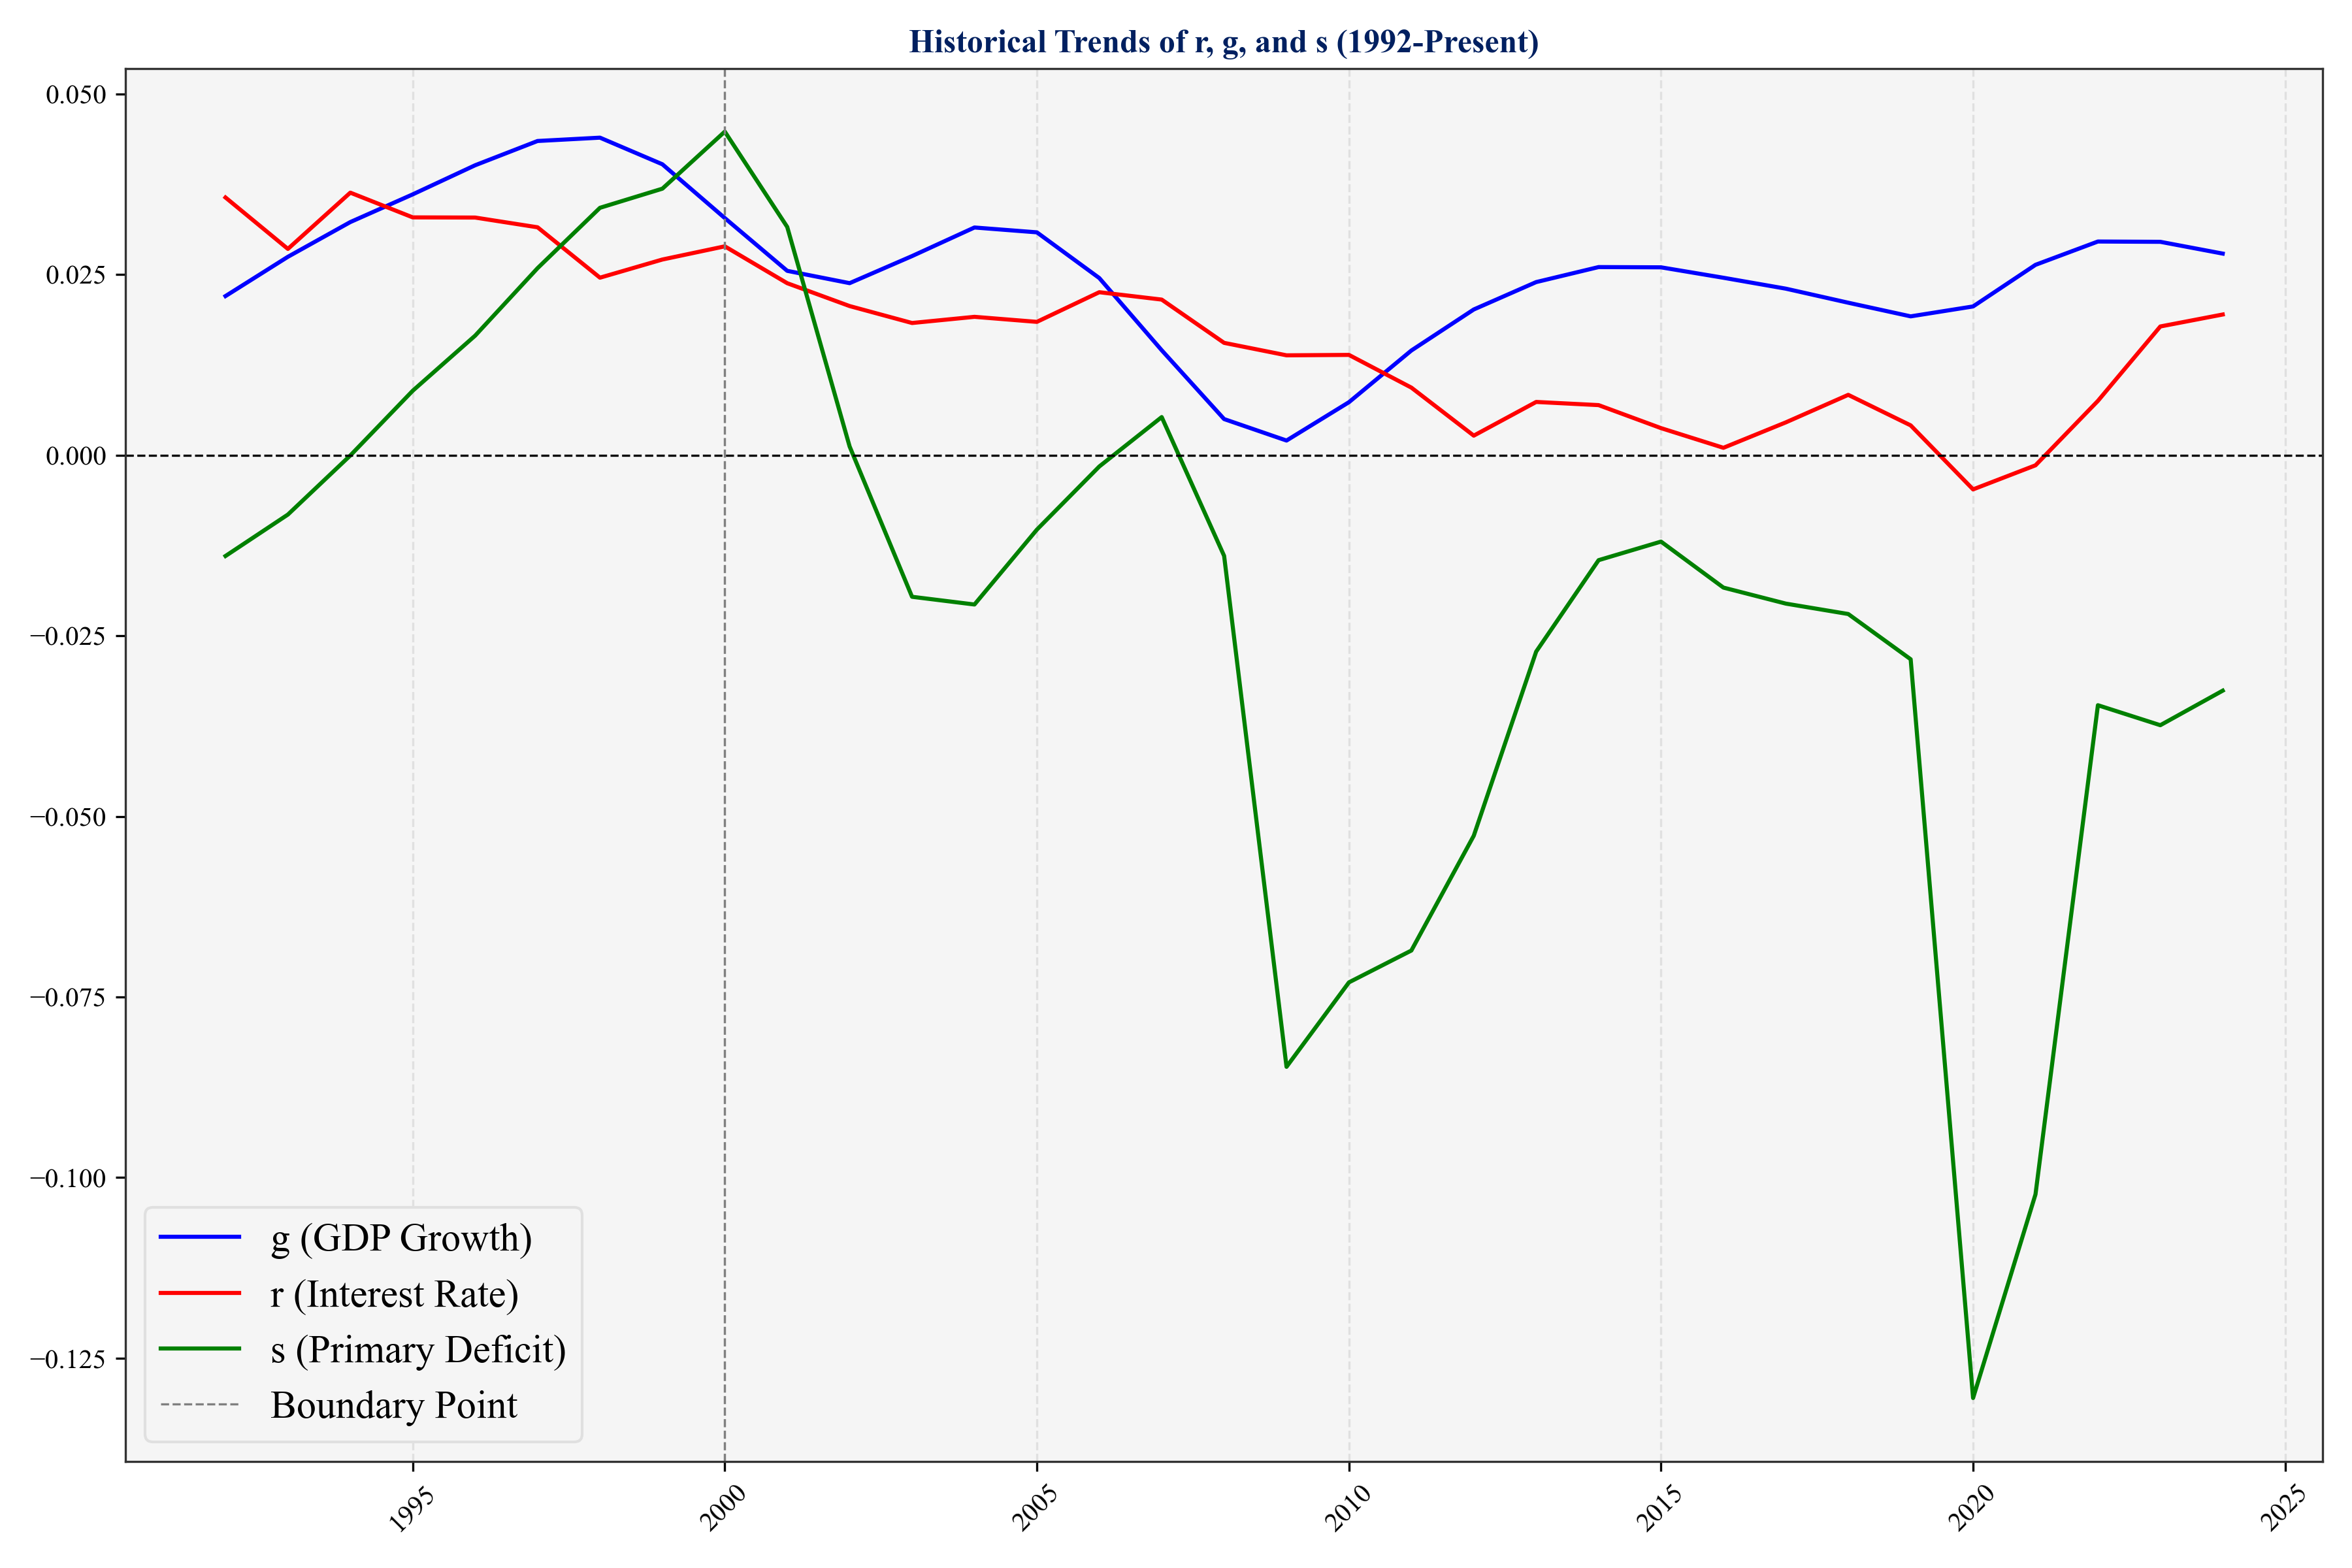
\includegraphics[width=0.65\textwidth]{historical_trends_rg_s.png}
	\caption{Historical Trends in $r$, $g$, and $s$}
\end{figure}

With this in hand, I make the following other decisions for model calibration. In addition to running two scenarios, one for an ``irresponsible" fiscal regime ($c = 0.33$) and the other for a ``responsible" fiscal regime ($c = 0.67$), I run three scenarios for $r-g$. In all three scenarios, $x_0 = 0$. Then, I model futures in which 1) growth consistently outpaces interest rates ($a_ u = \bar{r - g} = -0.01$ for data from 2000 onwards, during which $g > r$ consistently), 2) growth holds steady with interest rates ($a_u = 0$), and 2) growth falls behind interest rates ($a_u = - \bar{r-g}$ for data from 2000 onwards). 

Then, I estimate the standard deviation parameters $s_x$, $s_u$, and $s_s$ differently. 
First, I let $s_x = 1\%$ and $s_s = 1\%$.
Second, for $s_u$, I estimate the standard deviation in the observations of gap between the difference in $r-g$ from 2000 onwards to $\bar{r-g}$ and set this to equal $s_u$. From this, I have that $s_u = 1.85\%$.
These are admittedly rough approaches, but I think yield sensible results. 

\subsection{Model Results}

% Group 1
\begin{figure}[hbpt!]
\centering
\begin{subfigure}[b]{0.45\textwidth}
    \includegraphics[width=\textwidth]{sdsa_debt_random_walk_responsible.png}
    \caption{Responsible Regime - Debt Level Projections}
\end{subfigure}
\hfill
\begin{subfigure}[b]{0.45\textwidth}
    \includegraphics[width=\textwidth]{sdsa_debt_random_walk_irresponsible.png}
    \caption{Irresponsible Regime - Debt Level Projections}
\end{subfigure}

\centering
\begin{subfigure}[b]{0.45\textwidth}
    \includegraphics[width=\textwidth]{sdsa_debt_random_walk_responsible_slope.png}
    \caption{Responsible Regime - Debt Path Slope Projections}
\end{subfigure}
\hfill
\begin{subfigure}[b]{0.45\textwidth}
    \includegraphics[width=\textwidth]{sdsa_debt_random_walk_irresponsible_slope.png}
    \caption{Irresponsible Regime - Debt Path Slope Projections}
\end{subfigure}
\end{figure}

\begin{figure}[hbpt!]
\centering
\begin{subfigure}[b]{0.45\textwidth}
    \includegraphics[width=\textwidth]{sdsa_debt_random_walk_responsible_curvature.png}
    \caption{Responsible Regime - Debt Path Curvature Projections}
\end{subfigure}
\hfill
\begin{subfigure}[b]{0.45\textwidth}
    \includegraphics[width=\textwidth]{sdsa_debt_random_walk_irresponsible_curvature.png}
    \caption{Irresponsible Regime - Debt Path Curvature Projections}
\end{subfigure}

\centering
\begin{subfigure}[b]{0.45\textwidth}
    \includegraphics[width=\textwidth]{sdsa_debt_random_walk_responsible_curvature_distribution.png}
    \caption{Responsible Regime - Distribution of Debt Path Curvature}
\end{subfigure}
\hfill
\begin{subfigure}[b]{0.45\textwidth}
    \includegraphics[width=\textwidth]{sdsa_debt_random_walk_irresponsible_curvature_distribution.png}
    \caption{Irresponsible Regime - Distribution of Debt Path Curvature}
\end{subfigure}
\label{fig:debt_paths_all}
\end{figure}

\clearpage

\section{Estimation Approach 3 - Treating First Moment of Variables' Paths as Exogenous}

\subsection{Modeling Joint Distributions of $r$, $g$, and $s$}

\clearpage

\section{Appendix}

\subsection{Illustrating Debt Dynamics - A Basic Example}
\label{sec:appendix1}

To illustrate these equations in practice and start operationalizing \textit{sustainability}, I run two basic simulations below, the results (level, slope, and curvature) are plotted in Figure \ref{fig:debt_dynamics}. The logic of these simulations are simple. First, in Subfigure \ref{subfig:debt_dynamics_1}, I fix the three macroeconomic variables to be constant over the 30-year horizon, and model $b$, or debt, according to the Equation \ref{eq:b_basic}. Then, I run four scenarios:
\begin{center}
\begin{tabularx}{\textwidth}
  {>{\centering\arraybackslash}X
   >{\centering\arraybackslash}X
   >{\centering\arraybackslash}X
   >{\centering\arraybackslash}X}
 \textbf{Line Number (Color) } & $\mathbf{r}$ & $\mathbf{g}$ & $\mathbf{s}$ \\ \hline\hline
(1) (orange) & 0.04 & 0.02 & -0.02 \\
(2) (green) & 0.02 & 0.03 & -0.02 \\
(3) (pink) & 0.04 & 0.02 & 0.02 \\
(4) (brown) & 0.02 & 0.03 & 0.02 
\end{tabularx}
\end{center}

While the level of debt in the $r > g$ (deficit) would be of clear concern (reaching 250\% of GDP by year 30), the curvature of the line is negative in every year, albeit becoming less negative over time. In the other three scenarios, we can clearly identify non-explosive debt paths. This is, in one sense, unsurprising: the real concern of debt explosion / debt spiraling is the feedback loop between debt explosion and interest rates, the idea being that an increase in debt will increase interest rates. To incorporate this in these highly stylized simulations, in Subfigure \ref{subfig:debt_dynamics_2}, we can adopt a rule-of-thumb used in macroeconomic forecasting: a 1\% increase in debt leads to interest rates increasing by 2-3 basis points (in this simulation I use 2.5 basis points, or 0.0025\%). Incorporating this assumption into the simulation, the results are very different. We can see that the debt level explodes, but \textit{only} for the orange, or $r > g$ (deficit) scenario. Now, in contrast to the static simulations, however, we \textit{do} see explosions in curvature and slope, while the path for slope and curvature remain very similar for the other scenarios. 

\begin{figure}[htbp!]
\centering
	\begin{subfigure}[b]{0.45\textwidth}
		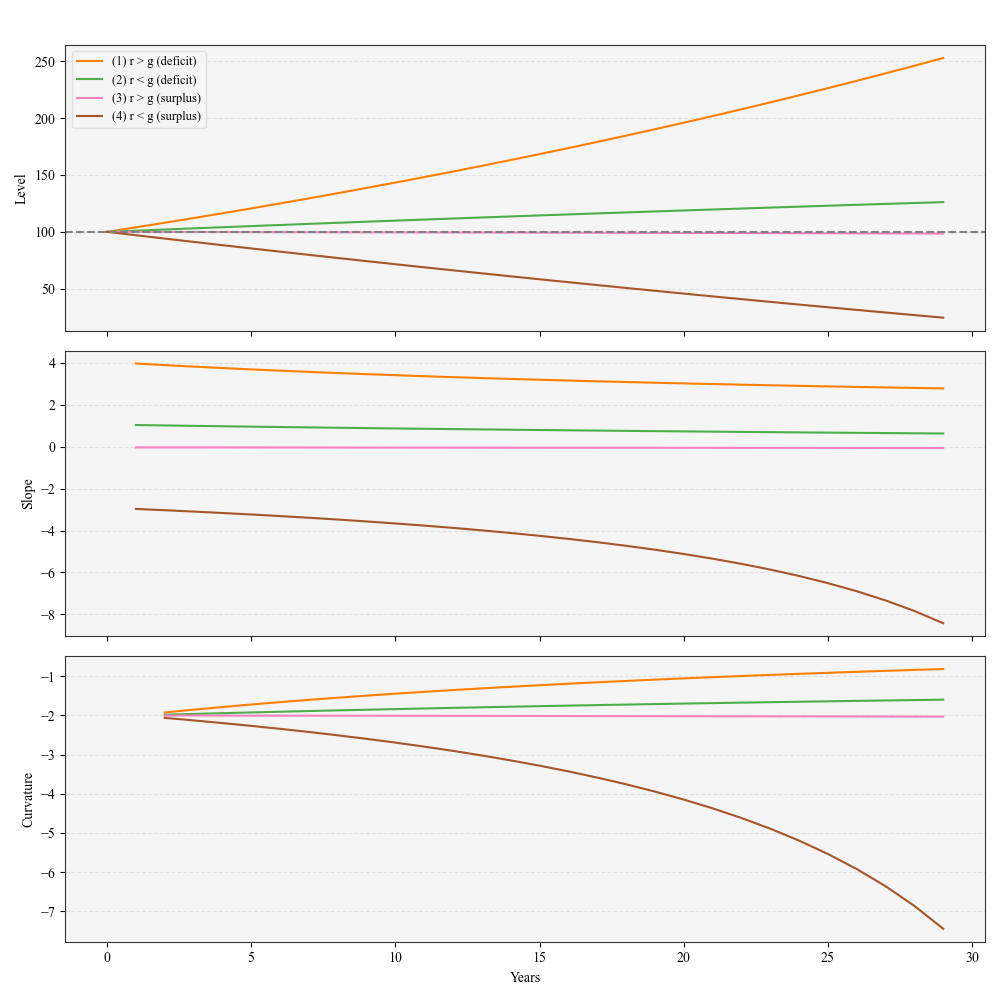
\includegraphics[width=\textwidth]{illustrative_debt_dynamics_1.png}
		\subcaption{Static $r$, $g$, and $s$}
		\label{subfig:debt_dynamics_1}
	\end{subfigure}
	\hfill
	\begin{subfigure}[b]{0.45\textwidth}
		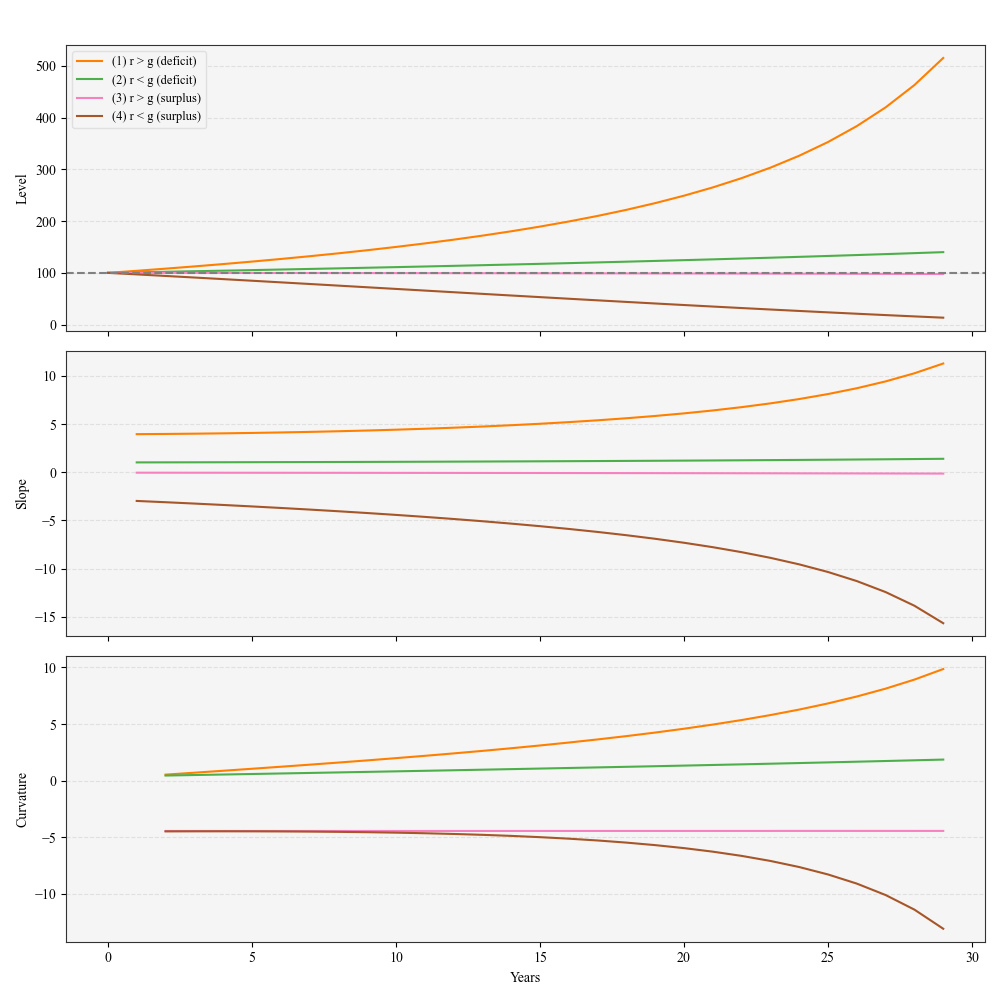
\includegraphics[width=\textwidth]{illustrative_debt_dynamics_2.png}
		\subcaption{Static $g$ and $s$, with feedback effect on $r$}
		\label{subfig:debt_dynamics_2}
	\end{subfigure}
	\caption{Illustrative Debt Dynamics: Two Scenarios}
	\label{fig:debt_dynamics}
\end{figure}

\subsection{Choosing $x_0$ and $a_u$}
\label{sec:xt_au_toggling}

We can alter this assumption by either toggling $x_0$ or $a_u$. To understand how these affect the values for $r-g$, I run the following scenarios through the model (holding $c = 0.5$ and maintaining all other assumptions of the model above):
\begin{center}
\begin{tabularx}{\textwidth}
  {>{\centering\arraybackslash}X
   >{\centering\arraybackslash}X
   >{\centering\arraybackslash}X
   >{\centering\arraybackslash}X} 
 \textbf{Line Number (Color)} & $\mathbf{x_0}$ & $\mathbf{a_u}$ \\ \hline\hline
(1) (orange) & -0.02 & 0 \\
(2) (green) & 0 & -0.02 \\
(3) (pink) & -0.02 & -0.02 \\
(4) (brown) & 0.02 & 0 \\
(5) (purple) & 0 & 0.02 \\
(6) (yellow) & 0.02 & 0.02 
\end{tabularx}
\end{center}

Then, I plot the mean value for $r_t - g_t = x_t + u_t$ in Subfigure \ref{subfig:random_walk_mean_rg} and the mean value for $b_t$ in Subfigure \ref{subfig:random_walk_rg_debt}:
\begin{figure}[htbp]
	\centering
	\begin{subfigure}[b]{0.45\textwidth}
		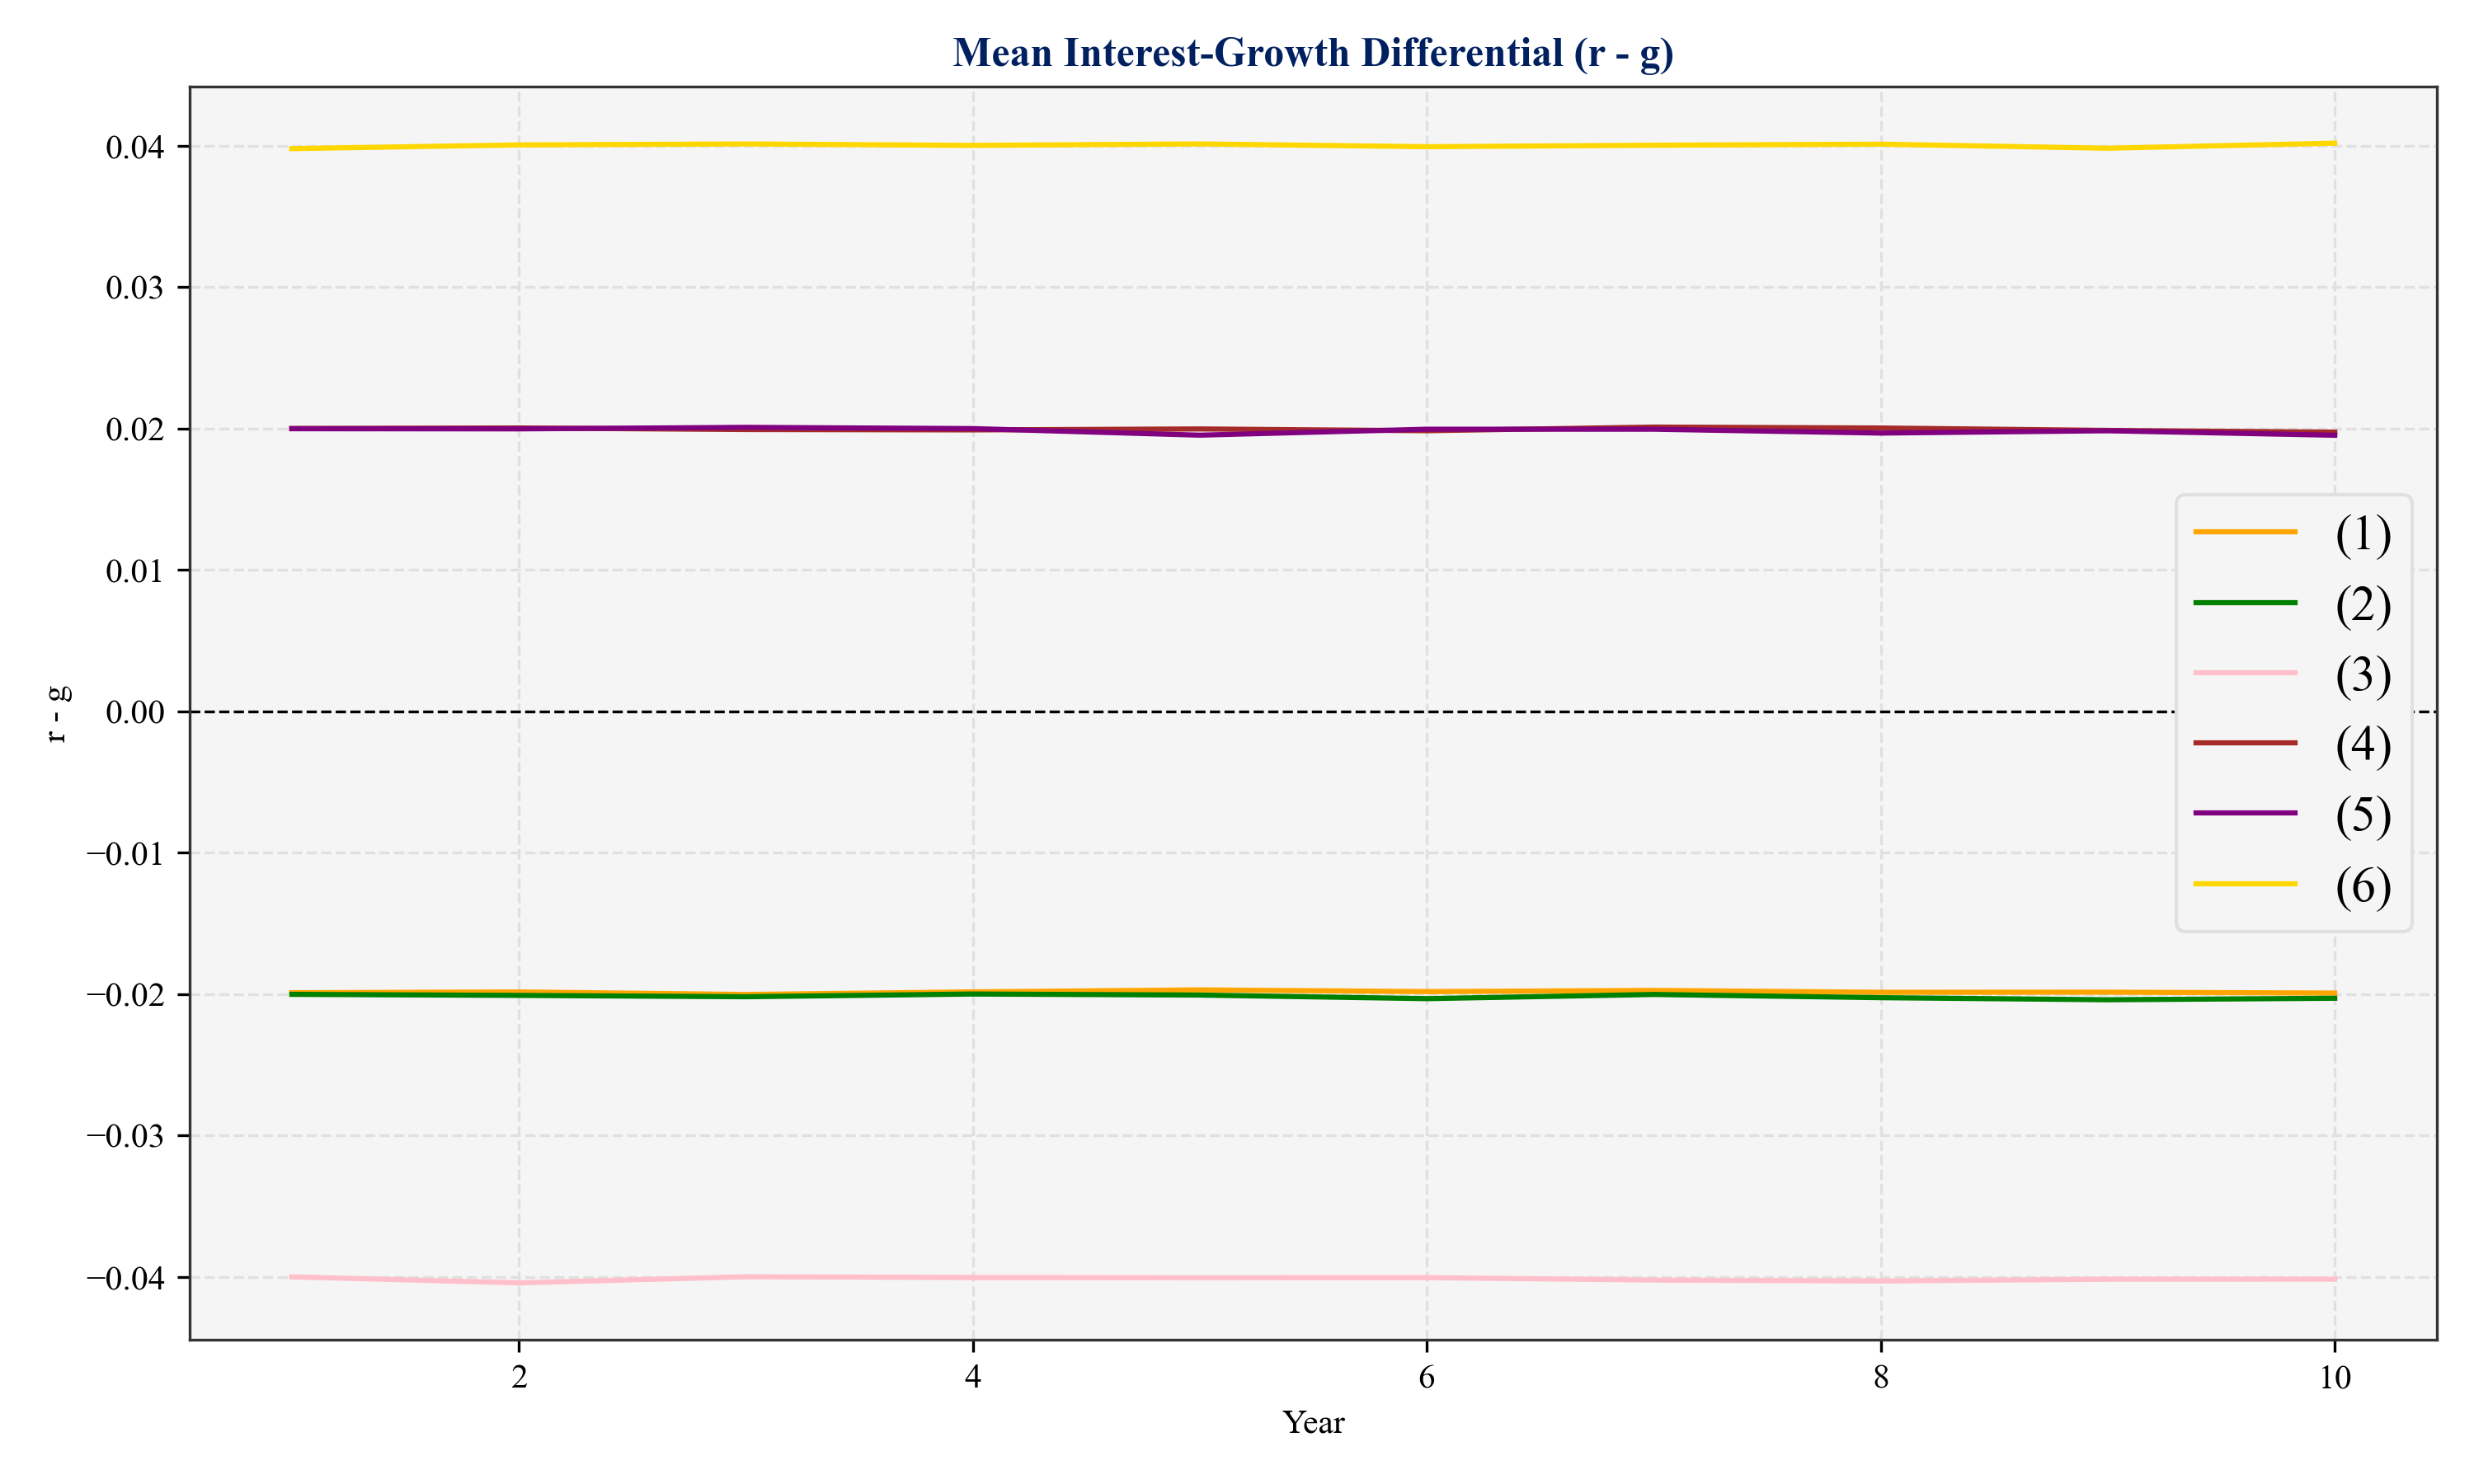
\includegraphics[width=\textwidth]{sdsa_random_walk_mean_rg.png}
		\caption{Distribution of 10-Year Debt Change}
		\label{subfig:random_walk_mean_rg}
	\end{subfigure}
	\hfill
	\begin{subfigure}[b]{0.45\textwidth}
		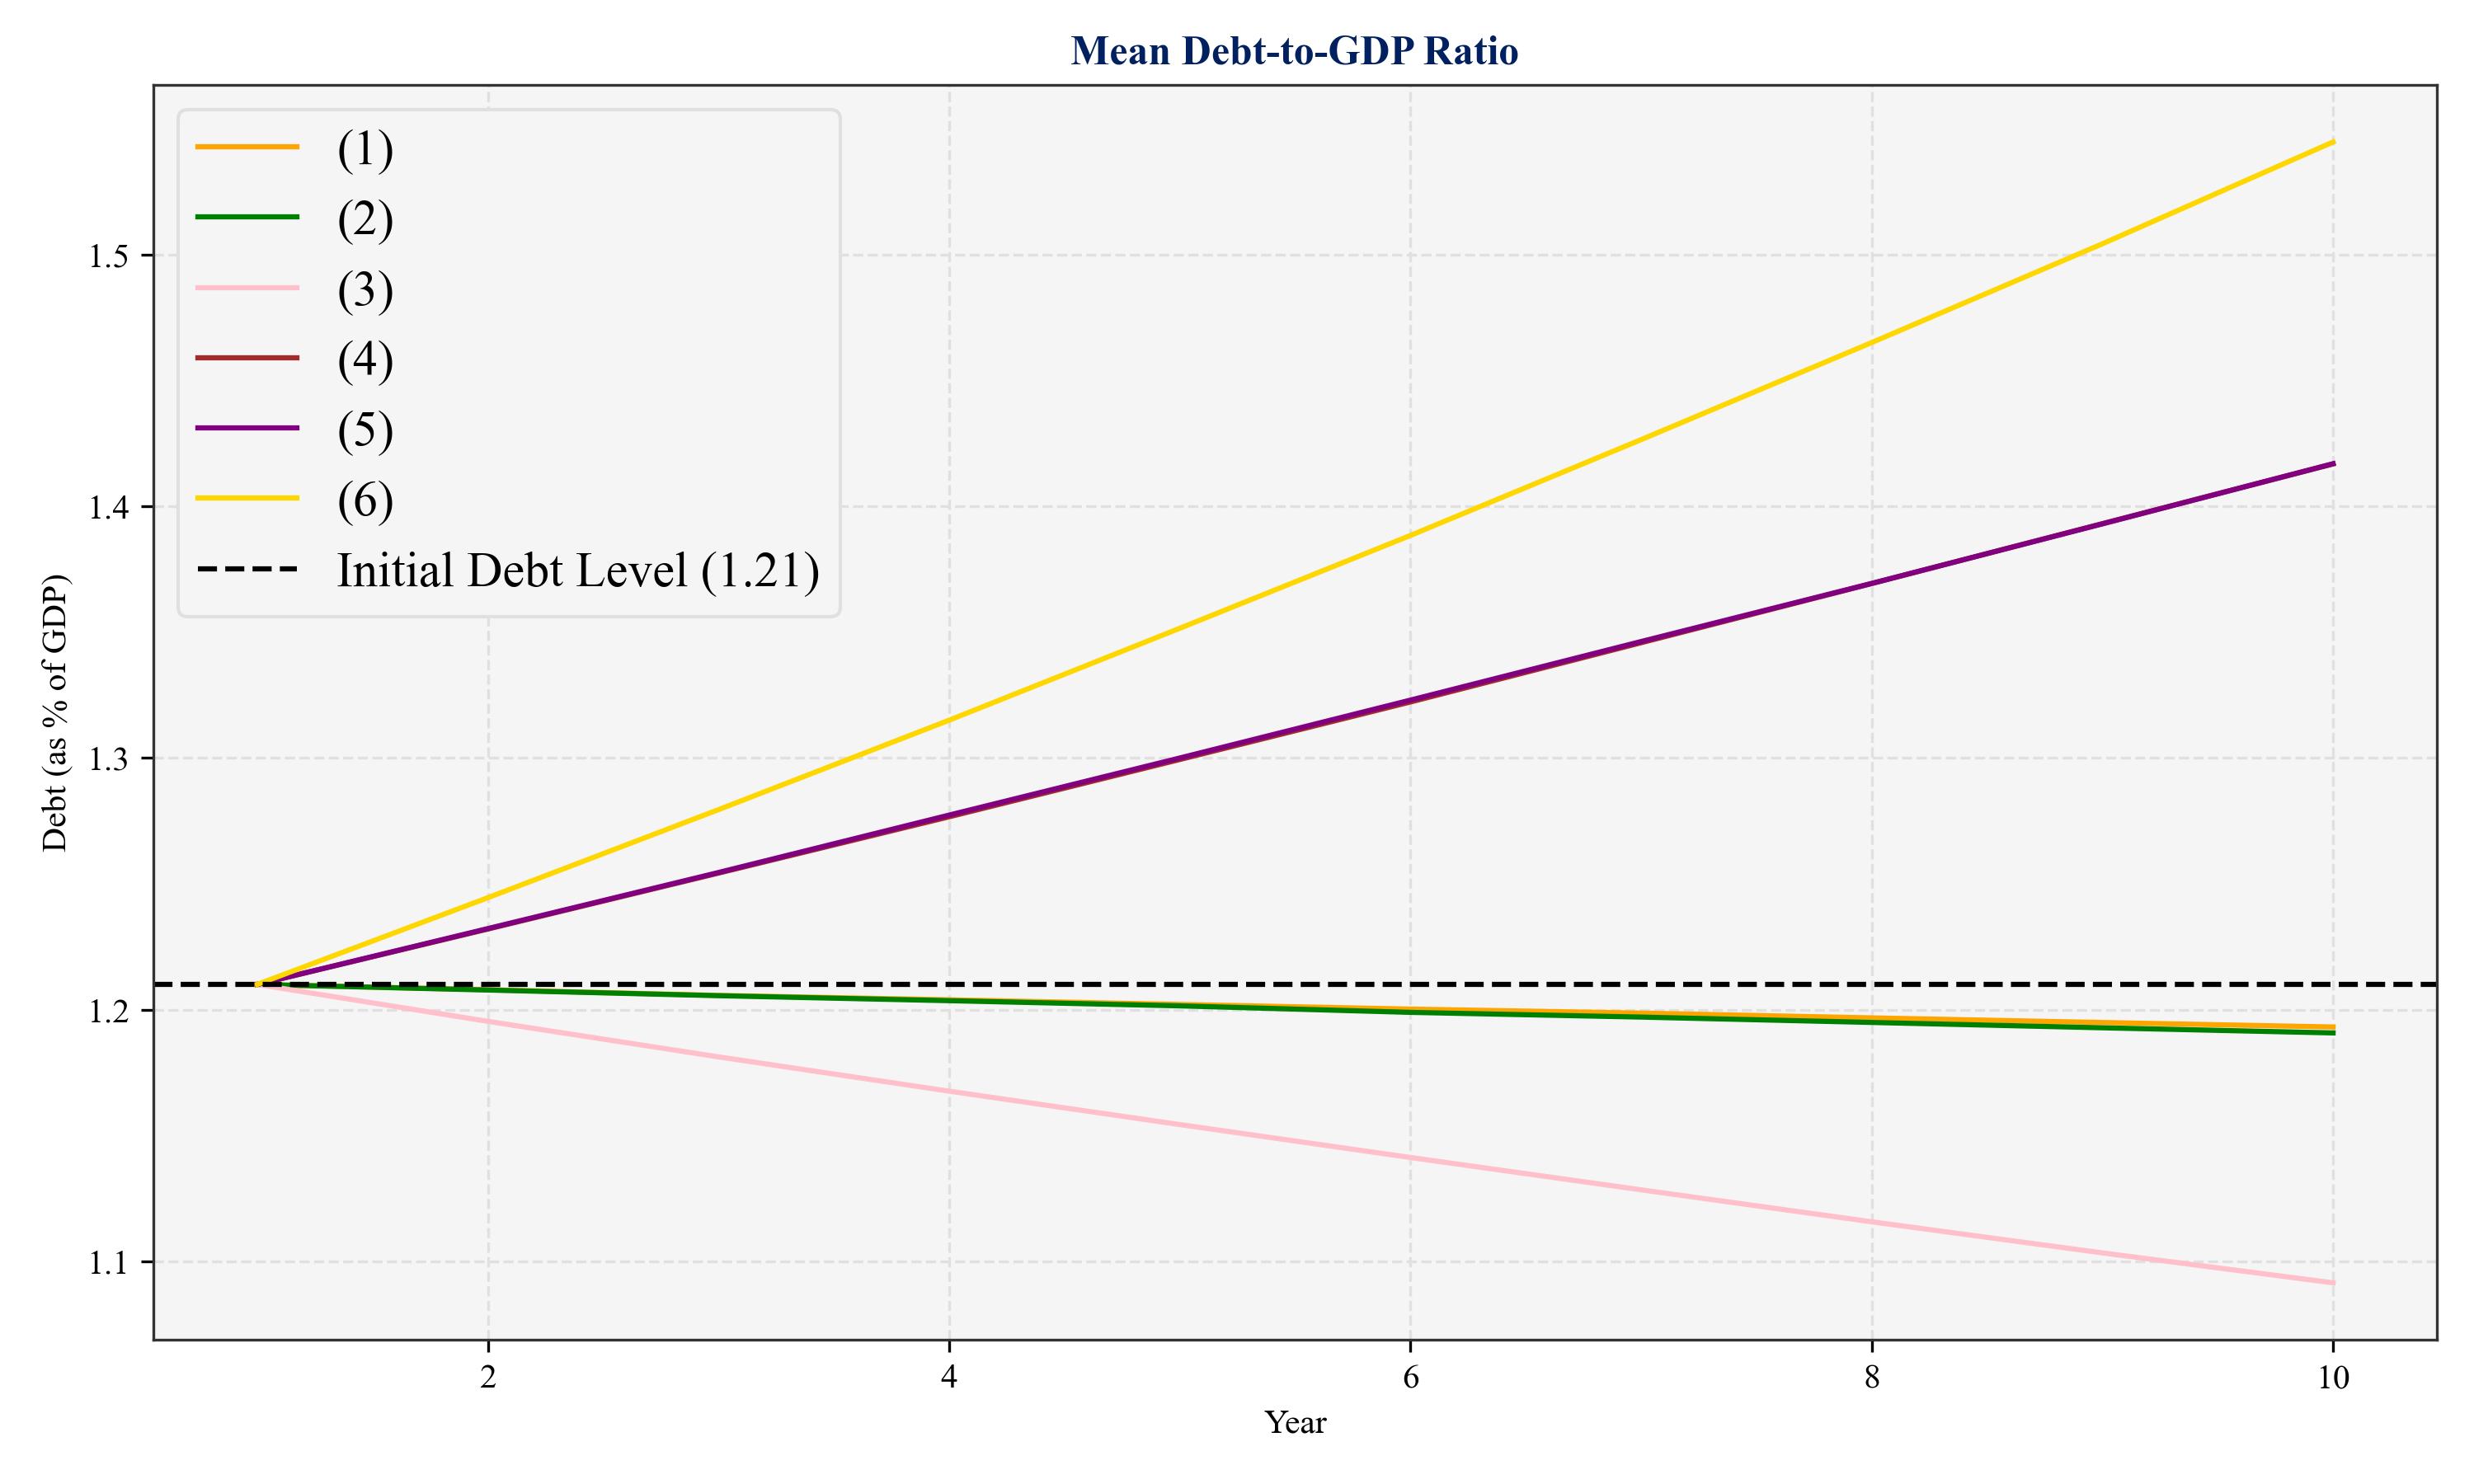
\includegraphics[width=\textwidth]{sdsa_random_walk_rg_varying_debt.png}
		\caption{Simulated Debt Paths}
		\label{subfig:random_walk_rg_debt}
	\end{subfigure}
	\caption{Simulated Debt Dynamics Under Varying Policy Feedback ($c$)}
	\label{fig:random_walk_varying_rg}
\end{figure}

Interestingly, there is practically no variation over time in the value of $r-g$; it appears our choices for $x_0$ and $a_u$ are fairly deterministic in setting the path of $r-g$ and -- as we see in Subfigure \ref{subfig:random_walk_rg_debt}, the setting of $r-g$ is deterministic in forecasting the path of debt. This SDSA model, then, is entirely dependent on how we pick $a_u$ and $x_0$, suggesting that the next iteration, which seeks to estimate the parameters based on historical data rather than set them as constants, will be more helpful and much more robust.

\subsection{Estimation Approach 1 - Calibration by Picking Constants}
\label{sec:sdsa_starter_random_walk}

The simplest and most straightforward approach for calibrating the SDSA model is by picking constant -- \textbf{this step does not involve estimation of parameters, rather the setting of parameters}. 

\subsection{Initial Assumptions for Calibration}

For the initial calibration I make the following assumptions:
\begin{itemize}
	\item $x_0 = 0$; this assumes that the persistent gap between $r$ and $g$ is fundamentally 0. The path of the \textit{persistent} component of this rate - growth gap, $x_t$, is then entirely subject to the random walks $e_t^x$. 
	\item $s_x = 0.3\%$; then, the variance accumulates linearly over $n$ periods, so that $\sigma(x_n)^2 = n \cdot s_x^2$, so that $\sigma(x_n) = \sqrt{n} \cdot s_x$. 
	\item $b_0 = 121\%$; this is roughly equal to the most up-to-date value for the debt-to-GDP ratio.
	\item $a_u = 0\%$; like our assumption that $x_0 = 0$, this assumption adopts a neutral stance towards the baseline or natural value for $r-g$.
	\item $s_u = 1\%$ and $s_s = 1\%$; these are generic assumptions of a seemingly reasonable standard deviation for the random walk / white noise process.
	\item $a_s = -2\%$; this could be interpreted as a `natural' or structural primary balance.
\end{itemize}

Then, I ran 5,000 simulations for each value of $c$ (0, 0.33, 0.67, and 1.0) to find detailed distributions of the key variables. Then, in Subfigure \ref{subfig:random_walk_distribution}, I plot the distribution of the 10-year level change in the debt level (as a share of GDP) among these four scenarios. In Subfigure \ref{subfig:random_walk_debt_path}, I  plot the 25th percentile, median, and 75th percentile of debt values by year among the simulations pertaining to each value of $c$. 
\begin{figure}[htbp]
	\centering
	\begin{subfigure}[b]{0.45\textwidth}
		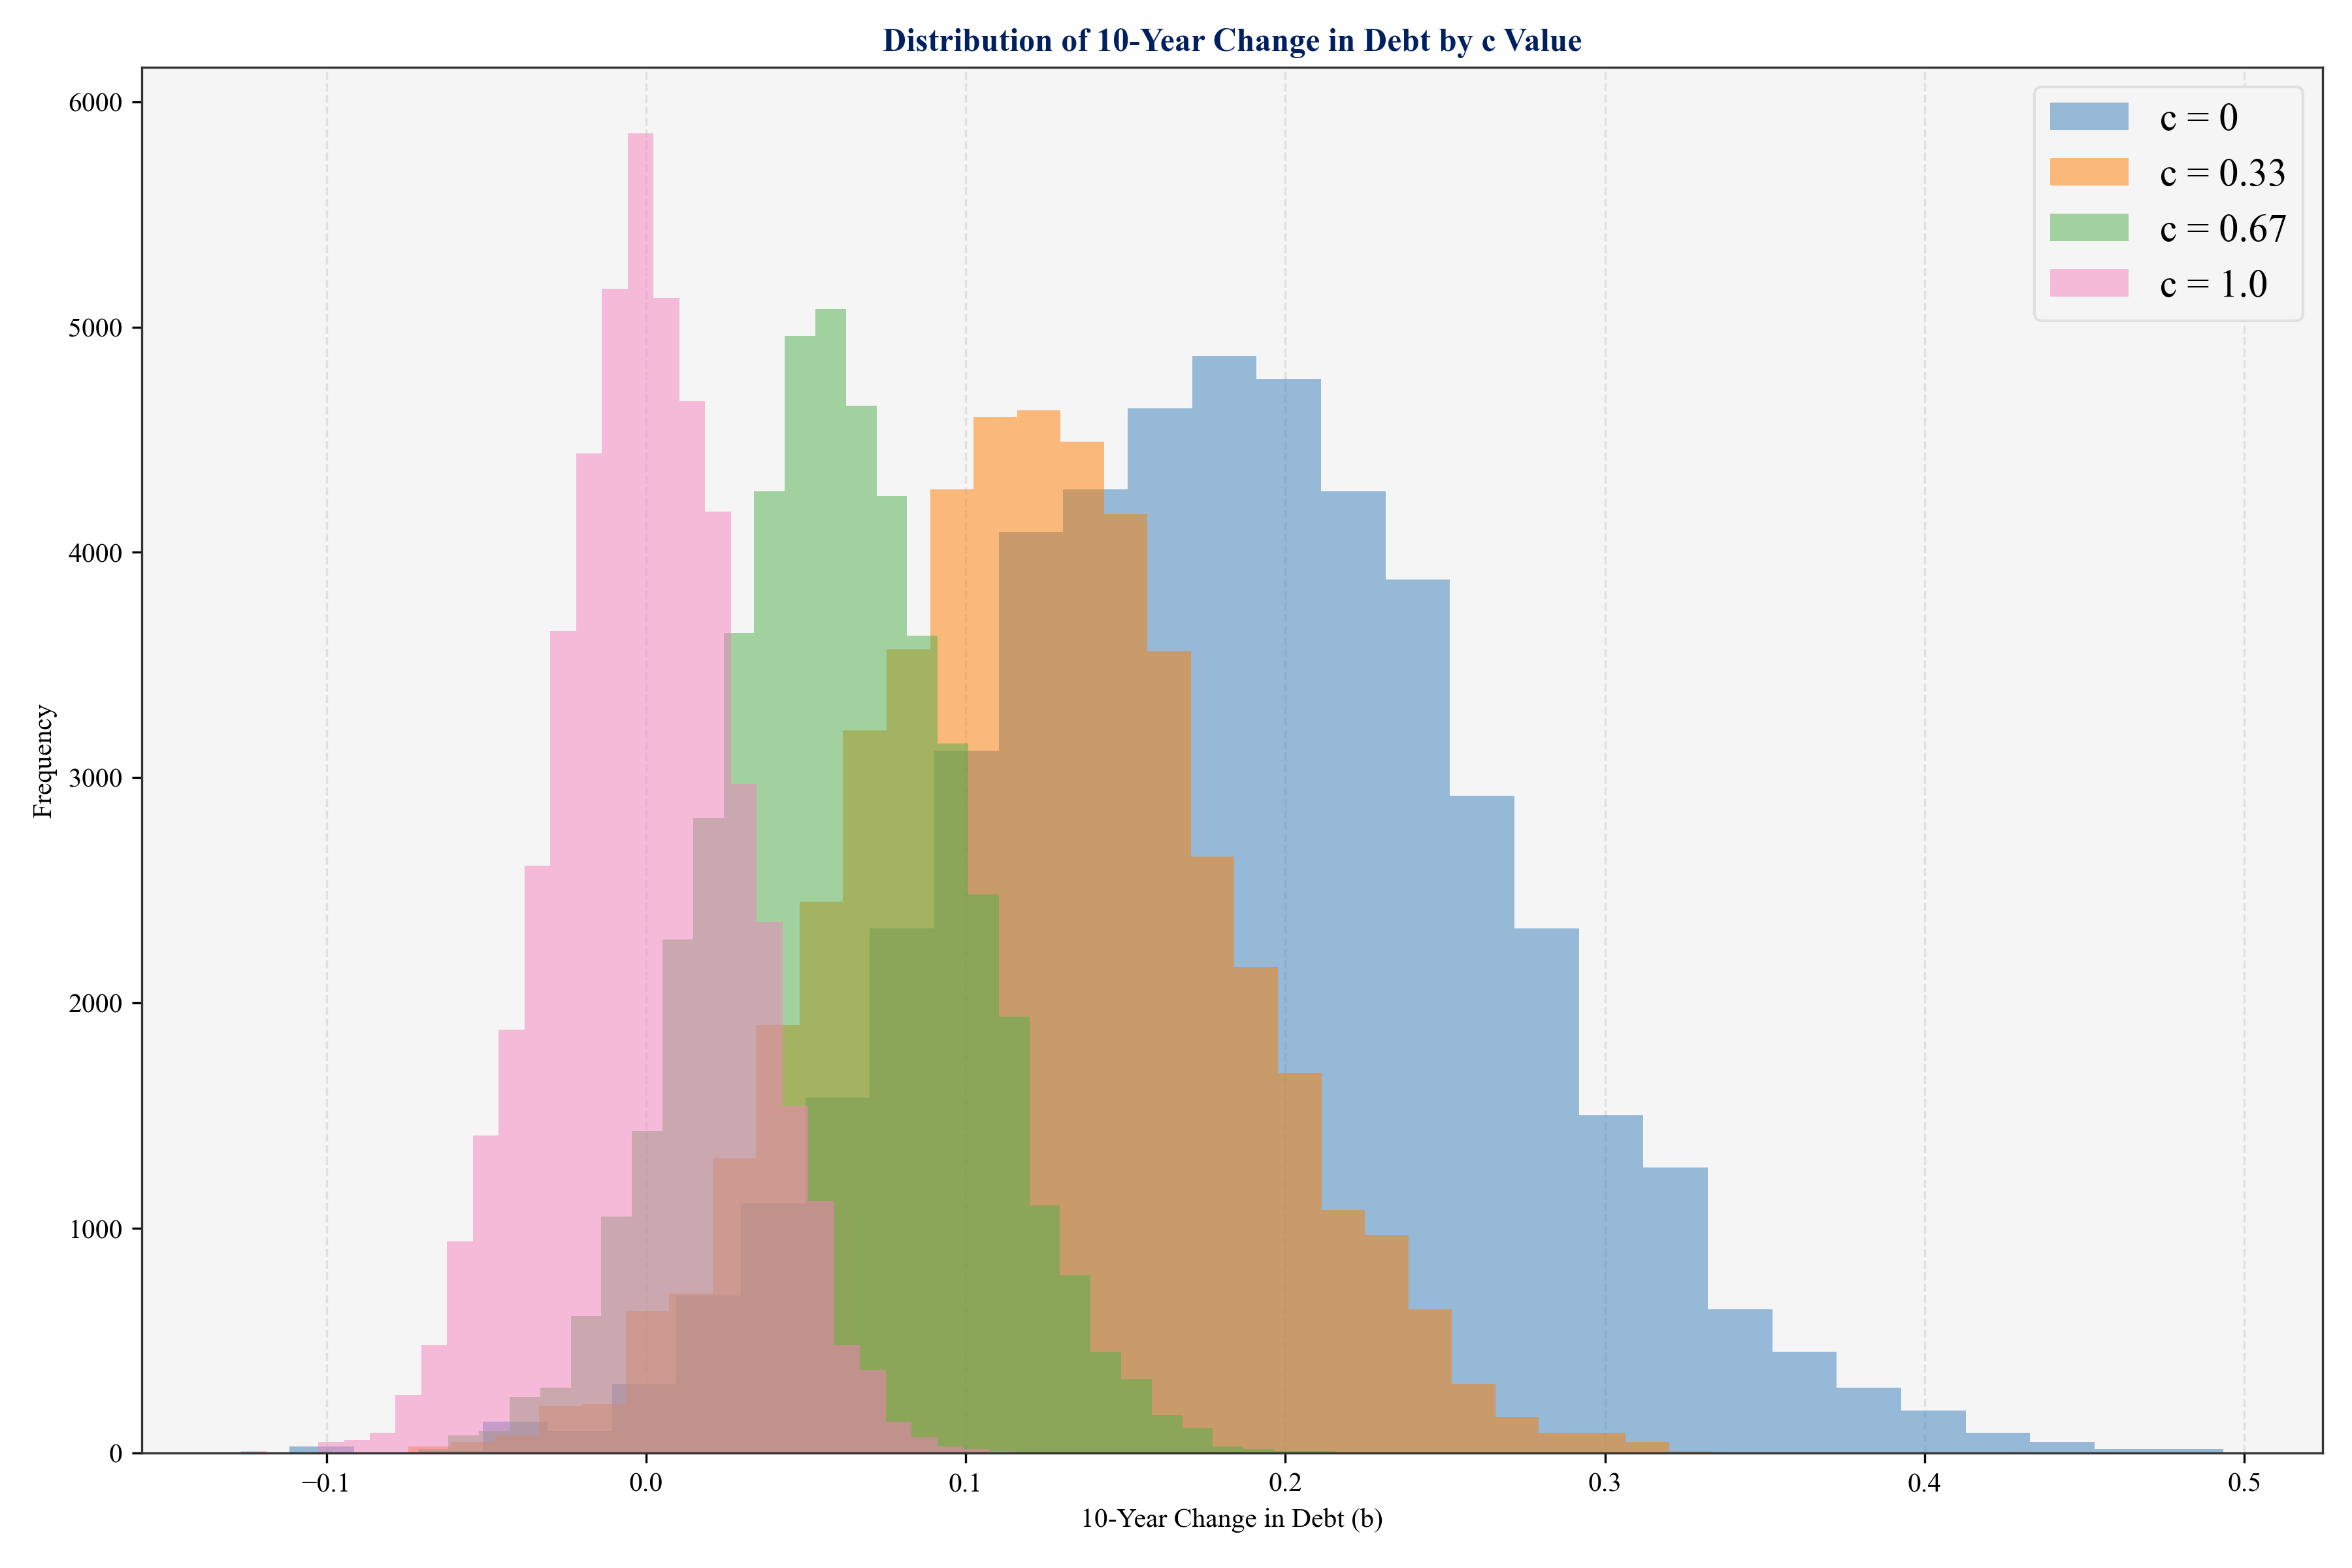
\includegraphics[width=\textwidth]{sdsa_debt_random_walk_distributions.png}
		\caption{Distribution of 10-Year Debt Change}
		\label{subfig:random_walk_distribution}
	\end{subfigure}
	\hfill
	\begin{subfigure}[b]{0.45\textwidth}
		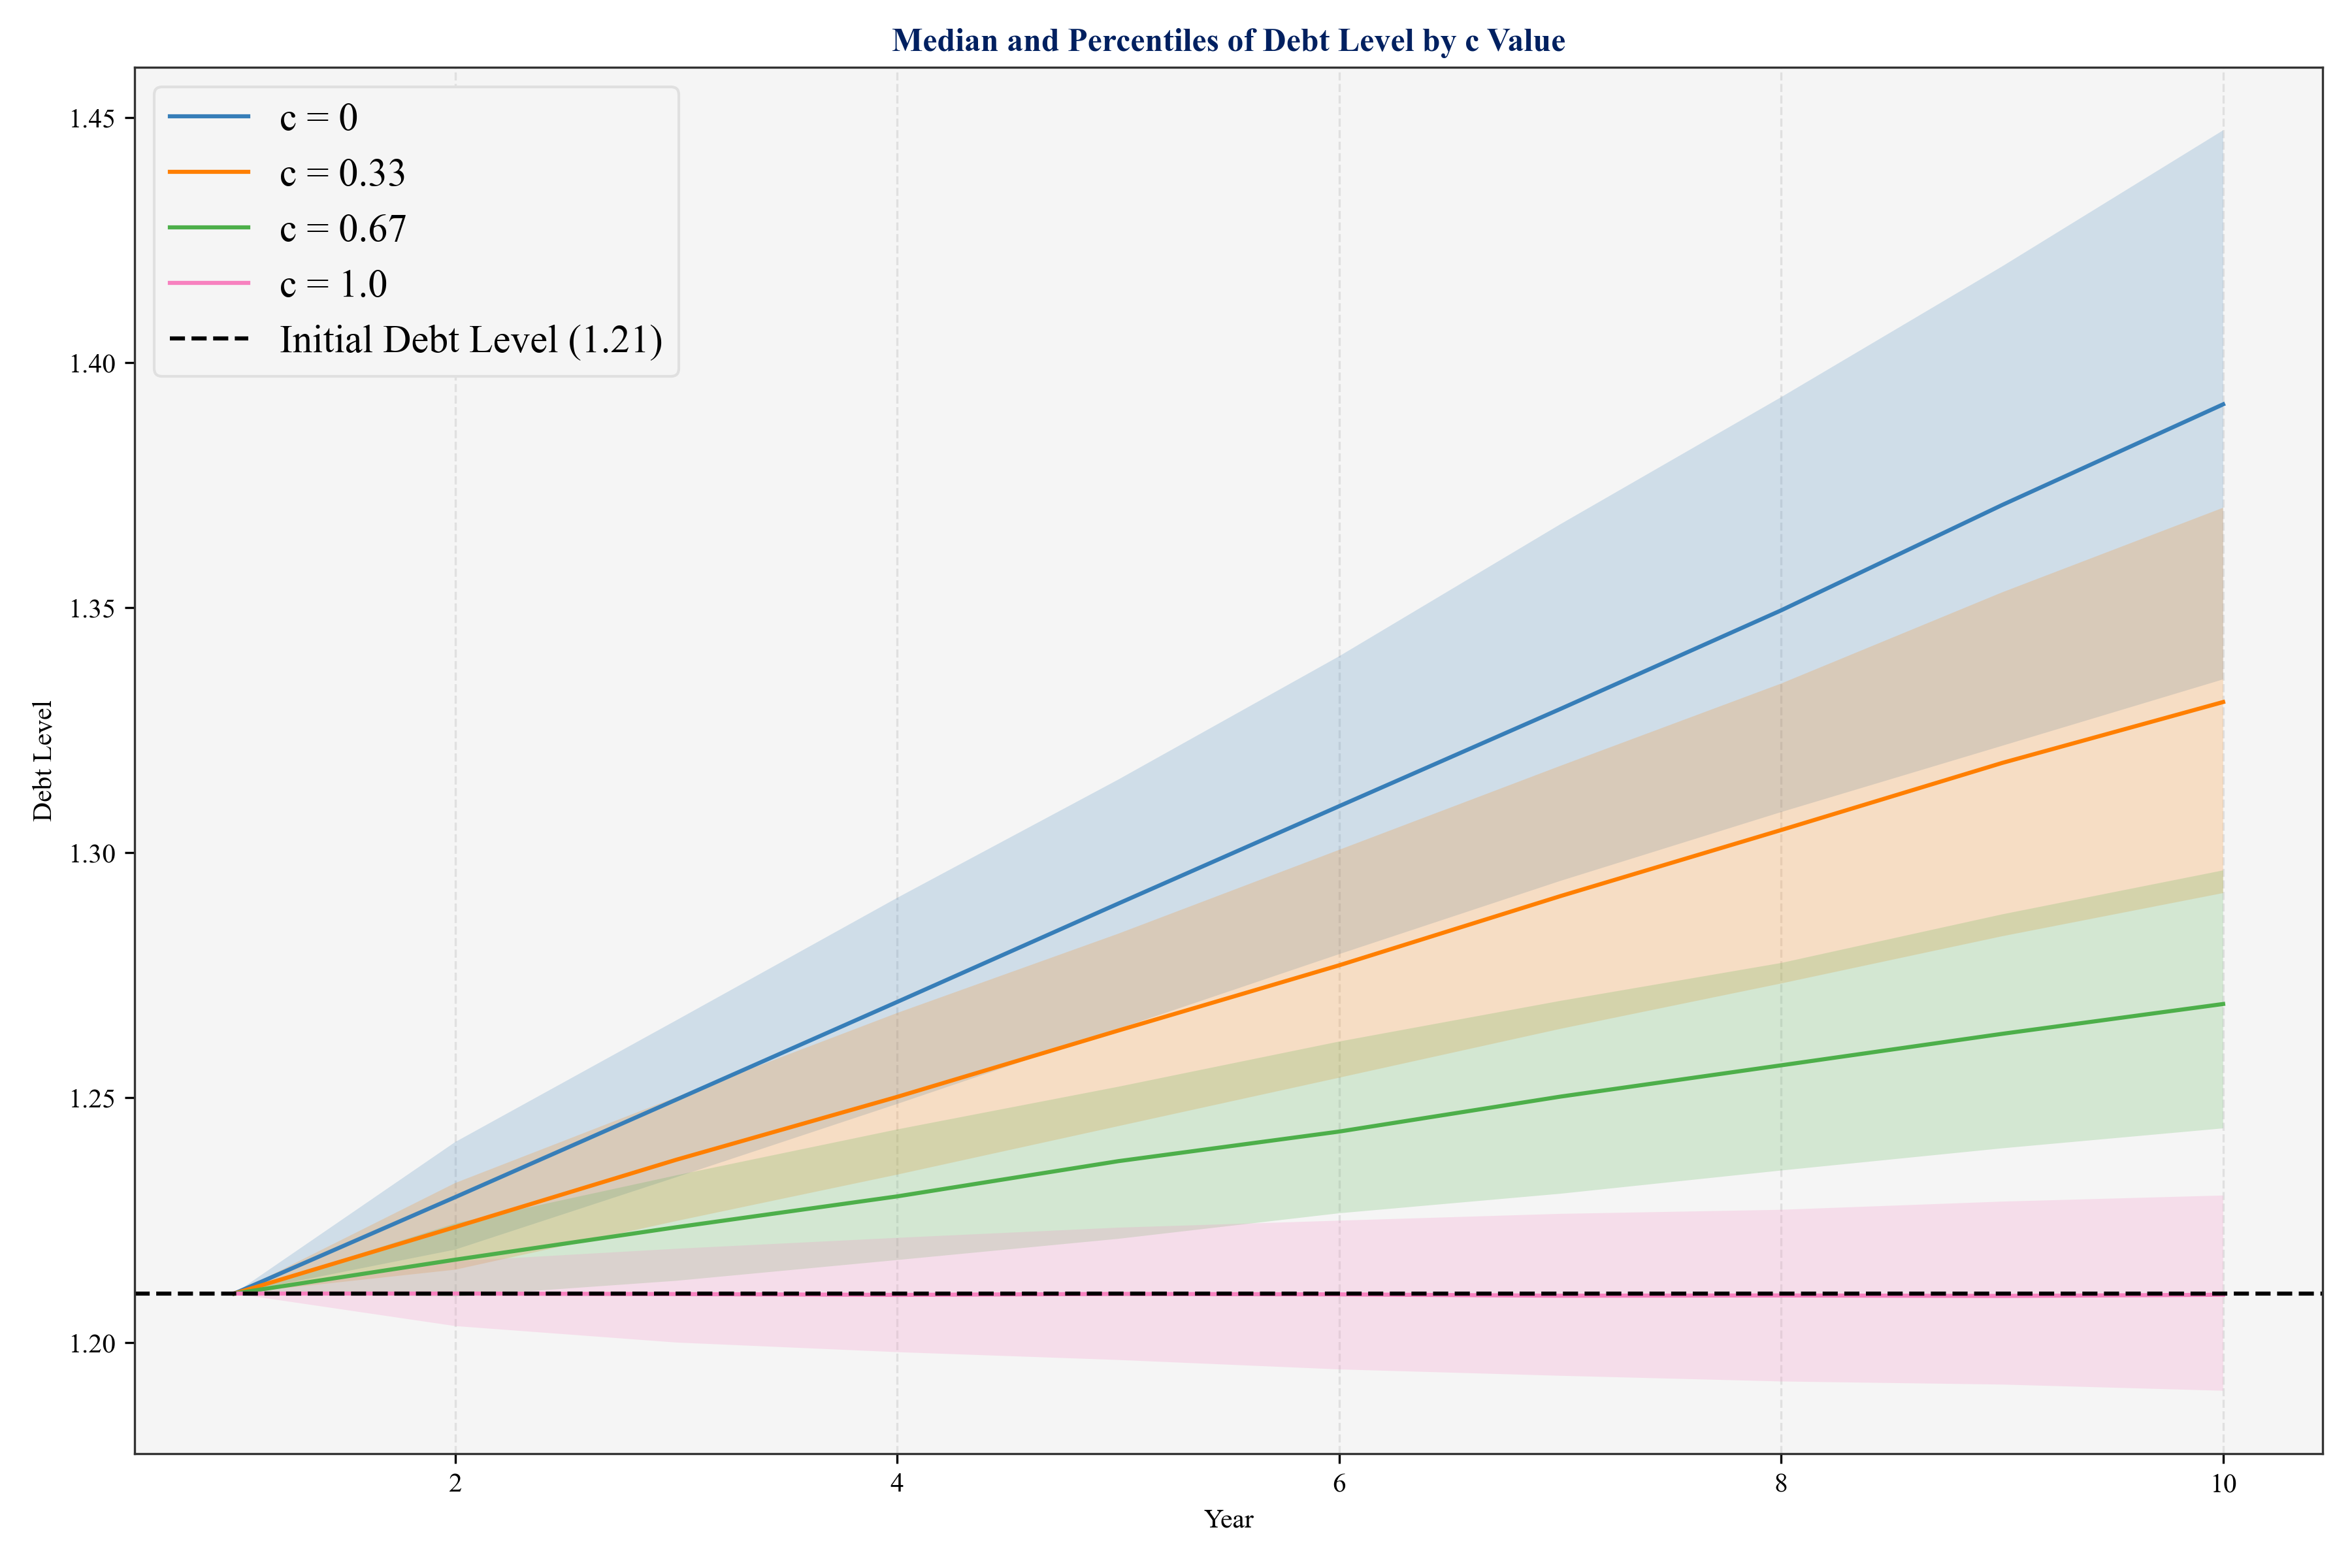
\includegraphics[width=\textwidth]{sdsa_debt_random_walk_path.png}
		\caption{Simulated Debt Paths}
		\label{subfig:random_walk_debt_path}
	\end{subfigure}
	\caption{Simulated Debt Dynamics Under Varying Policy Feedback ($c$)}
	\label{fig:random_walk_sdsa}
\end{figure}

These results illustrate a few core principles of our model are working properly. Importantly, $c$ is correctly calibrating the debt path; perfect policy feedback stabilizes the debt at its initial level and as policy becomes more unresponsive to debt (i.e., $c$ approaches 0), the steeper the slope of the debt path. Nonetheless, these results have a few serious shortcomings. The first and clearest is that its assumptions take a stance on the future path of $r-g$ by assuming that the baseline difference between $r$ and $g$ is 0. Of course, this might not be true. 

\subsection{Detailed Notes on Historical Data Choice}
\label{sec:detailed_historical_data}

Given that some versions of our model will require the use of historical data in modeling correlation between macroeconomic variables. I want to be clear where historical is coming from. First, we are presented with a basic choice in finding data for $r$, $g$, and $s$: should we use the expected values of this data (i.e., copying Blanchard's Figure 3.3), or observed values of this data. 

Blanchard uses data from the Federal Reserve Bank of Philadelphia's \href{https://www.philadelphiafed.org/surveys-and-data/real-time-data-research/survey-of-professional-forecasters}{Survey of Professional Forecasters} (SPF), specifically following: $r = (10-\text{yr nominal yields} - \text{SPF forecasts of 10 year inflation}$ and $g = \text{SPF forecasts of 10 year real growth rates}$. Alternatively, we can use observed historical data to estimate $r$ and $g$. Specifically, we can estimate $r$ by dividing the total interest outlay by the total debt owed by the federal government using Bureau of Economic Analysis (BEA) data and $g$ by using BEA GDP numbers with \href{https://fred.stlouisfed.org/series/GDPDEF}{FRED's Implicit Price Deflator}. Then below in Figure \ref{fig:r_g_comparison}, I compare these two historical estimates of $r$ and $g$:
\begin{figure}[htbp]               % placement for the whole float
  \centering                       % centre the two subfigures as a block
  \begin{subfigure}{0.48\textwidth}% width of this sub-box
    \centering
    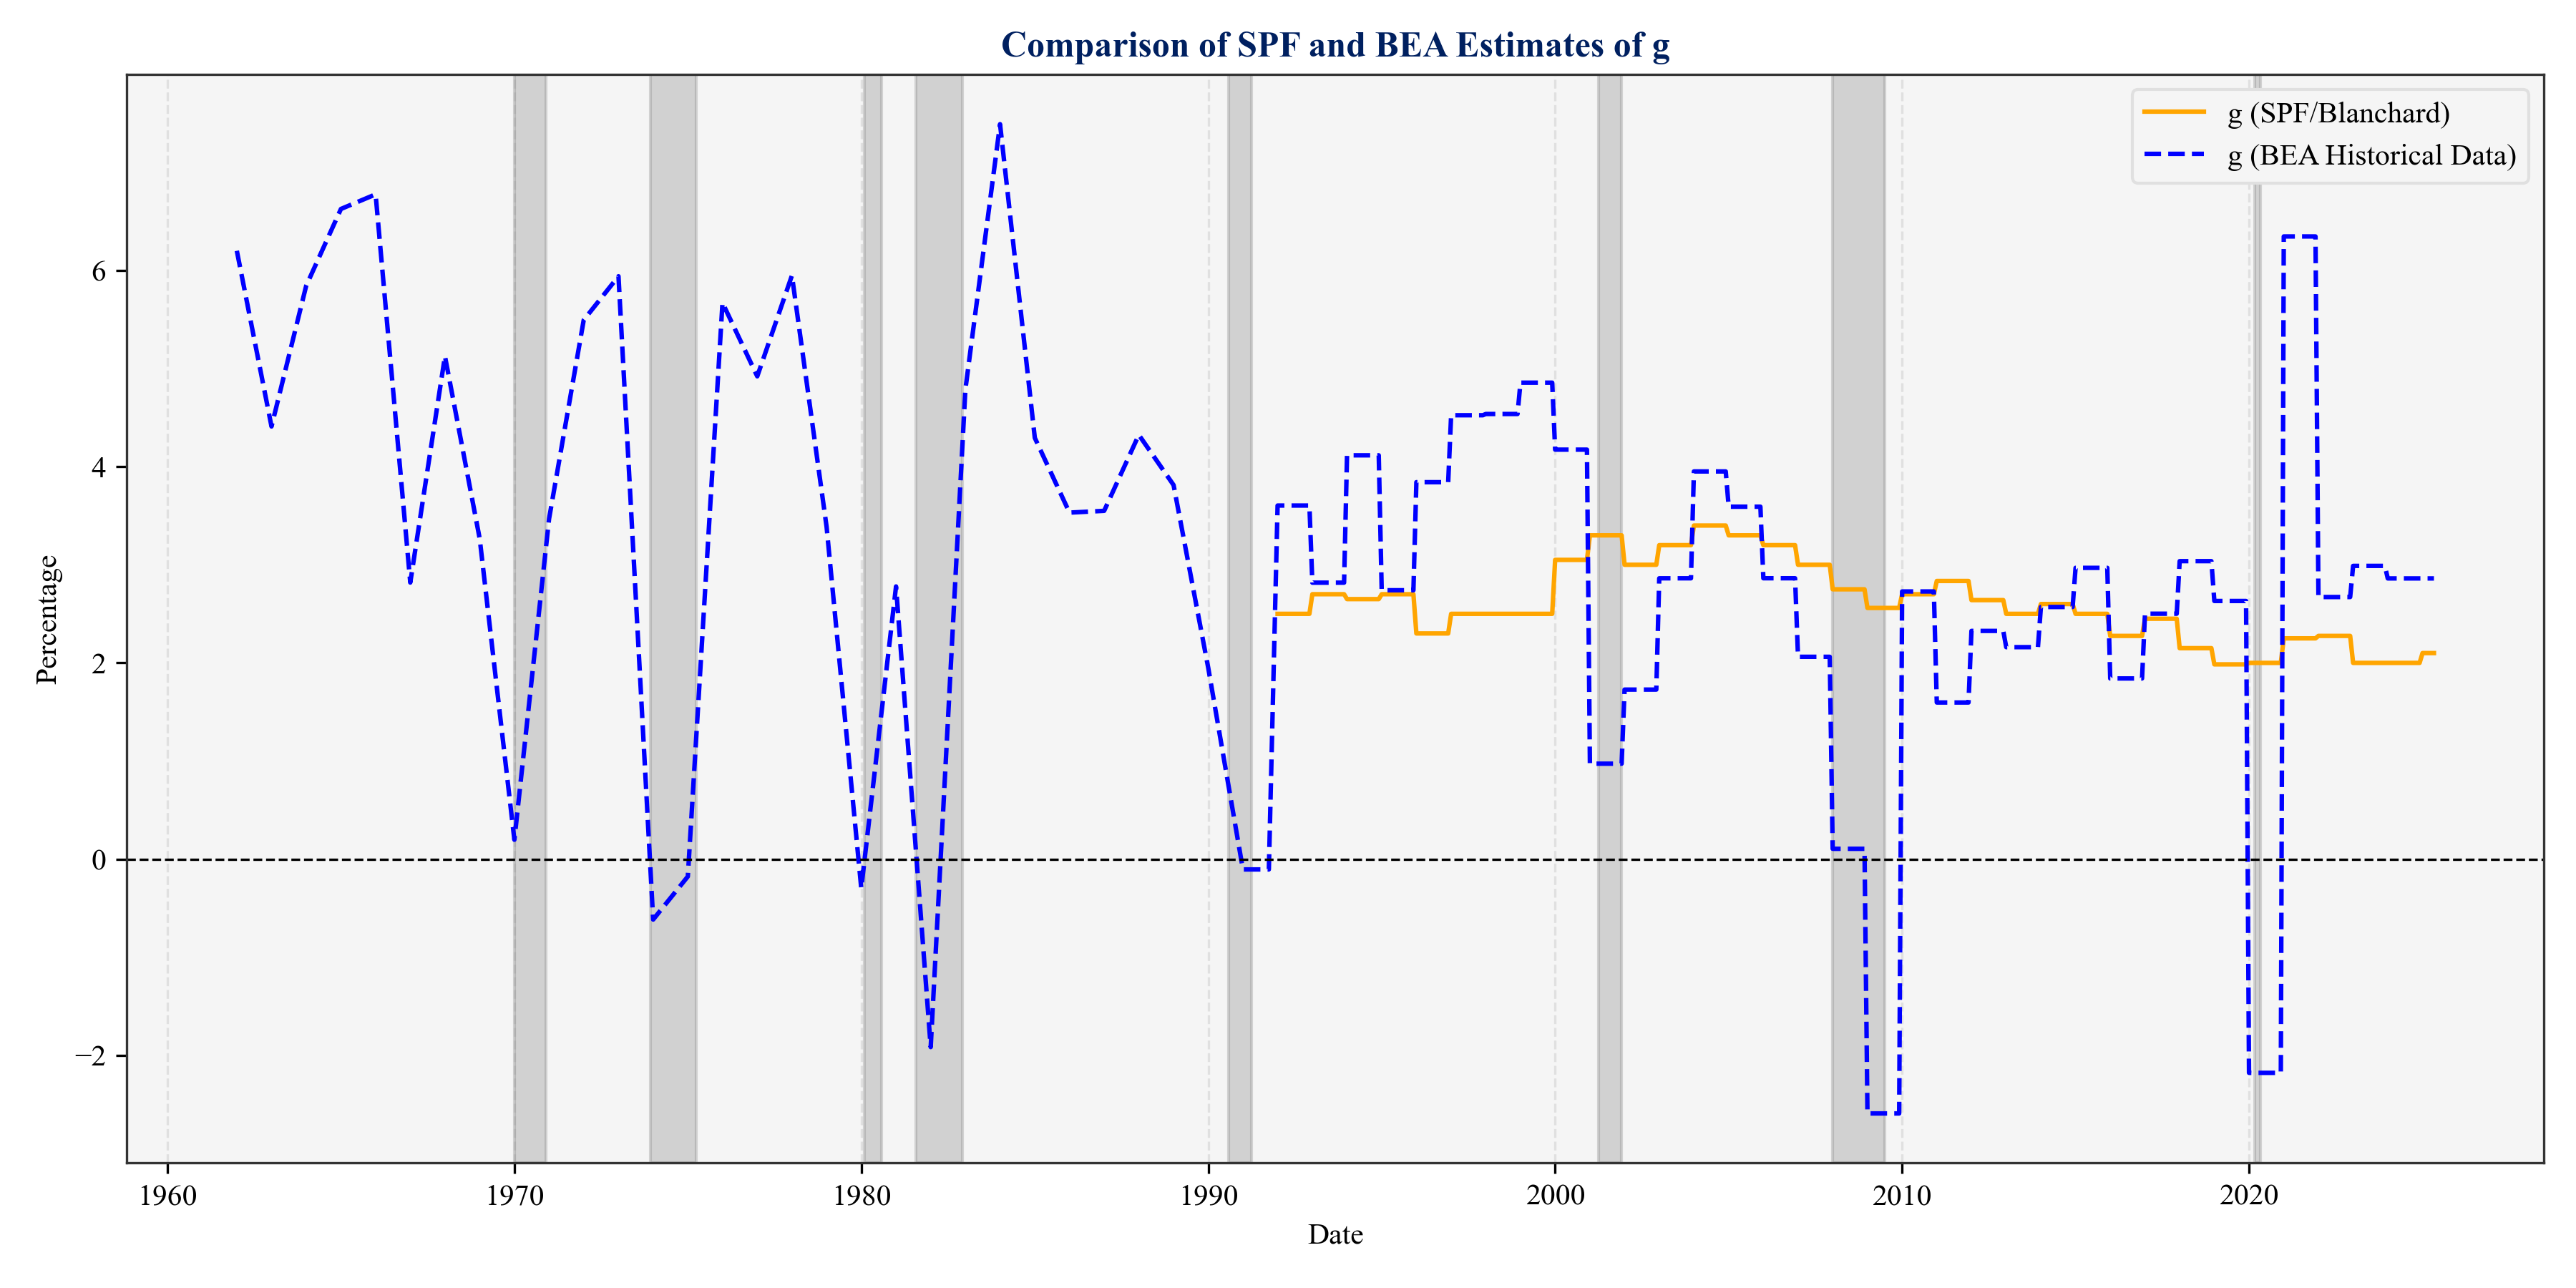
\includegraphics[width=\linewidth]{g_comparison.png}
    \caption{$g$ estimates}        % caption for (a)
    \label{subfig:g_comparison}
  \end{subfigure}
  \hfill                             % horizontal space between the two
  \begin{subfigure}{0.48\textwidth}
    \centering
    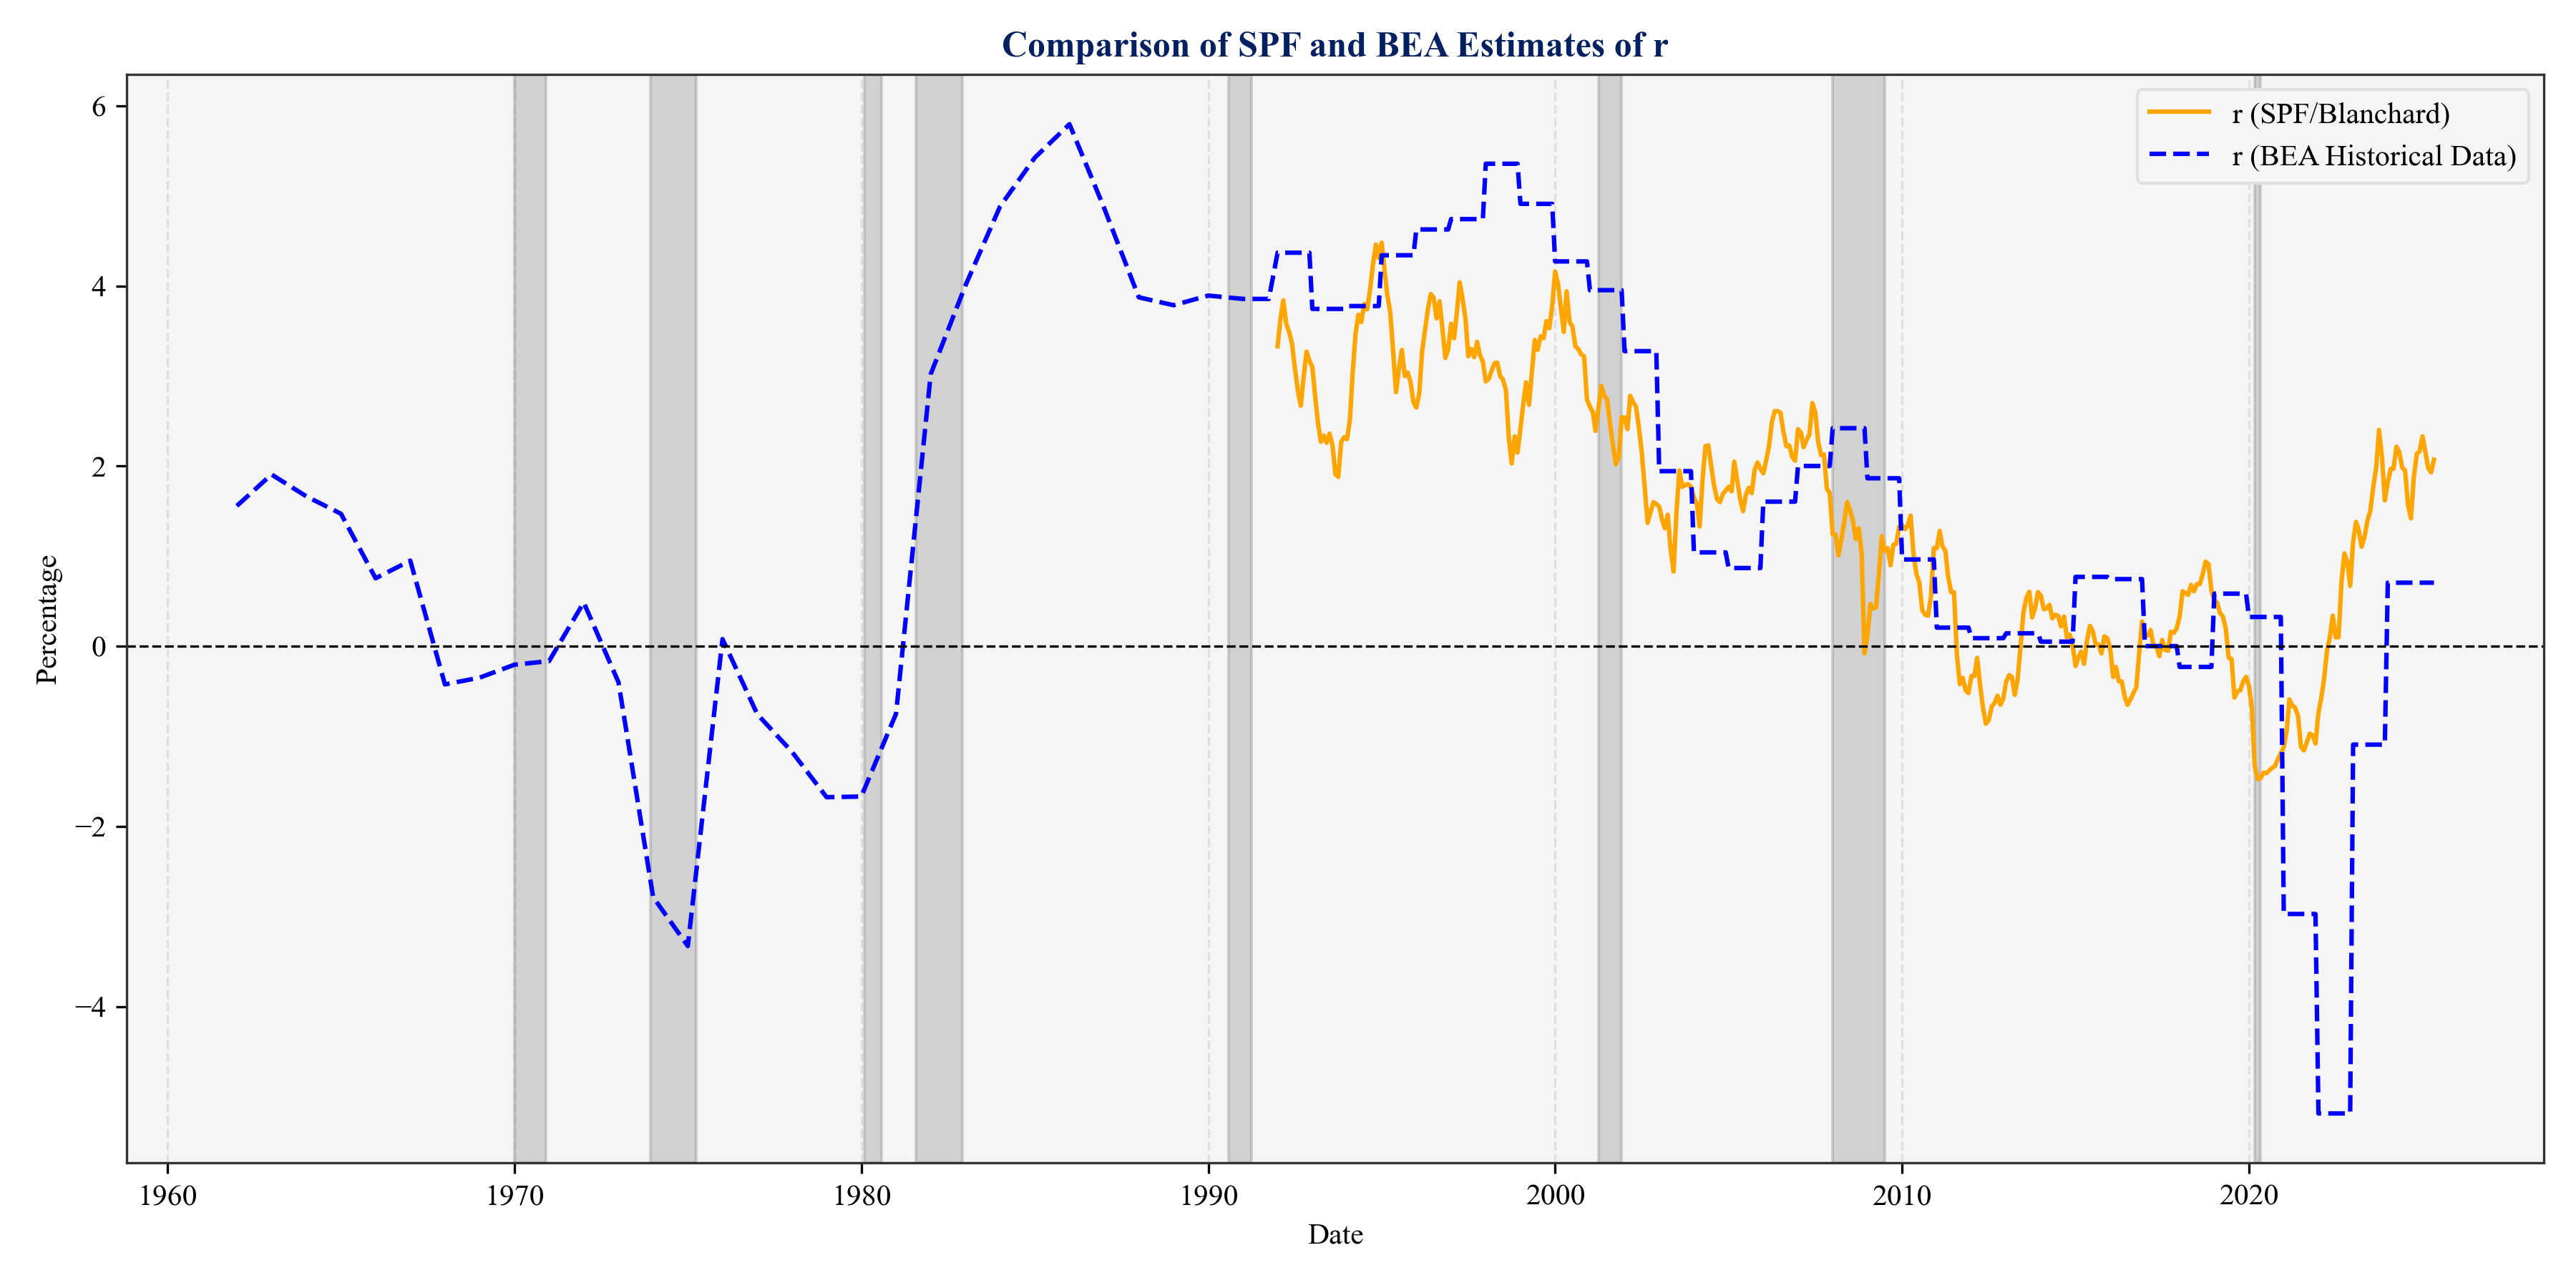
\includegraphics[width=\linewidth]{r_comparison.png}
    \caption{$r$ estimates}
    \label{subfig:r_comparison}
  \end{subfigure}
  \caption{The two approaches yield broadly similar trajectories for
           $r$ and $g$, though the implied volatility differs.}
  \label{fig:r_g_comparison}
\end{figure}

Substantively, these two approaches also mean different things. Blanchard uses the 10-year forecasts from the Survey of Professional Forecasts; thus, the $g$ from SPF is the annualized 10-year growth rate, necessarily much more stable / flat than the annual growth rate. $r$ on the other hand tracks much more closely between the two approaches, in large part because Blanchard uses the observed 10-year nominal yield and the forecasted inflation rate. 

\subsection{Detailed Information on Forecasts}

First, here are a set of forecasts for $r$, the \textbf{real interest rate}. 
\begin{center}
\begin{threeparttable}
\begin{tabularx}{\textwidth}{>{\centering\arraybackslash}X >{\centering\arraybackslash}X >{\centering\arraybackslash}X}
  \textbf{Source} & \textbf{Policy Context / Assumption} & \textbf{Horizon} \\ \hline\hline
  \href{https://budgetlab.yale.edu/research/financial-cost-senate-passed-budget-bill}{Budget Lab (Yale)\tnote{a}} & Senate-passed budget bill & 30 years \\
  Mark Zandi, Moody's Analytics\tnote{b} & Tariffs\tnote{c} & 4 years, quarterly \\
  \href{https://www.cbo.gov/data/budget-economic-data\#3}{Congressional Budget Office (CBO)} & Baseline (January 2025) & 10 years, quarterly \\
\end{tabularx}

\vspace{1ex}
\begin{tablenotes}
\footnotesize
\item[a] “The Financial Cost of the Senate-Passed Budget Bill,” July 1, 2025.
\item[b] Not publicly available; provided directly to authors.
\item[c] These projections include three scenarios of future tariff policy:
\begin{itemize}
  \item \textbf{S1}: Return tariffs to pre-2025 levels starting 2025q3 and maintain.
  \item \textbf{S2}: 10\% reciprocal, 25\% steel/aluminum, 25\% auto, 30\% China (2025q3 onward).
  \item \textbf{S3}: 20\% reciprocal, 50\% steel/aluminum, 50\% auto, 50\% pharma/semi, 40\% China (2025q3 onward).
\end{itemize}
\end{tablenotes}
\end{threeparttable}
\end{center}
\vspace{0.15in}

Second, here are a set of forecasts for $g$, the \textbf{real GDP growth}:
\begin{center}
\begin{threeparttable}
\begin{tabularx}{\textwidth}{>{\centering\arraybackslash}X >{\centering\arraybackslash}X >{\centering\arraybackslash}X}
\textbf{Source} & \textbf{Policy Context / Assumption} & \textbf{Horizon} \\
\hline\hline
\href{https://budgetlab.yale.edu/research/state-us-tariffs-june-17-2025}{Budget Lab (Yale)\tnote{a}} & 2025 Tariffs, Against Baseline & 10 years, quarterly \\
Mark Zandi, Moody's Analytics\tnote{b} & Tariffs & 4 years, quarterly \\
\href{https://www.cbo.gov/data/budget-economic-data\#3}{Congressional Budget Office (CBO)} & Baseline (January 2025) & 10 years, quarterly \\
\end{tabularx}
\vspace{1ex}
\begin{tablenotes}
\footnotesize
\item[a] “State of U.S. Tariffs: June 17, 2025.”
\item[b] Not publicly available; provided directly to authors.
\end{tablenotes}
\end{threeparttable}
\end{center}

\vspace{0.15in}

Third, here are a set of forecasts for $s$, the \textbf{primary surplus} (or deficit):
\begin{center}
\begin{threeparttable}
\begin{tabularx}{\textwidth}{>{\centering\arraybackslash}X >{\centering\arraybackslash}X >{\centering\arraybackslash}X}
\textbf{Source} & \textbf{Policy Context / Assumption} & \textbf{Horizon} \\
\hline\hline
\href{https://budgetlab.yale.edu/research/financial-cost-senate-passed-budget-bill}{Budget Lab (Yale)\tnote{a}} & Senate-passed budget bill & 30 years \\
\href{https://www.cbo.gov/data/budget-economic-data\#3}{Congressional Budget Office (CBO)} & Baseline (January 2025) & 10 years \\
\end{tabularx}
\vspace{1ex}
\begin{tablenotes}
\footnotesize
\item[a] “The Financial Cost of the Senate-Passed Budget Bill,” July 1, 2025.
\end{tablenotes}
\end{threeparttable}
\end{center}

It is clear, as illustrated in Figures \ref{fig:forecasts_r}, \ref{fig:forecasts_g}, and \ref{fig:forecasts_s} that there is significant heterogeneity across these sources. It is clear that we have to make choices in selecting the forecasting source that we use for the first moment of the joint distributions of $r$, $g$, and $s$. 

\begin{figure}[htbp!]
\centering

\begin{subfigure}[b]{0.60\textwidth}
    \centering
    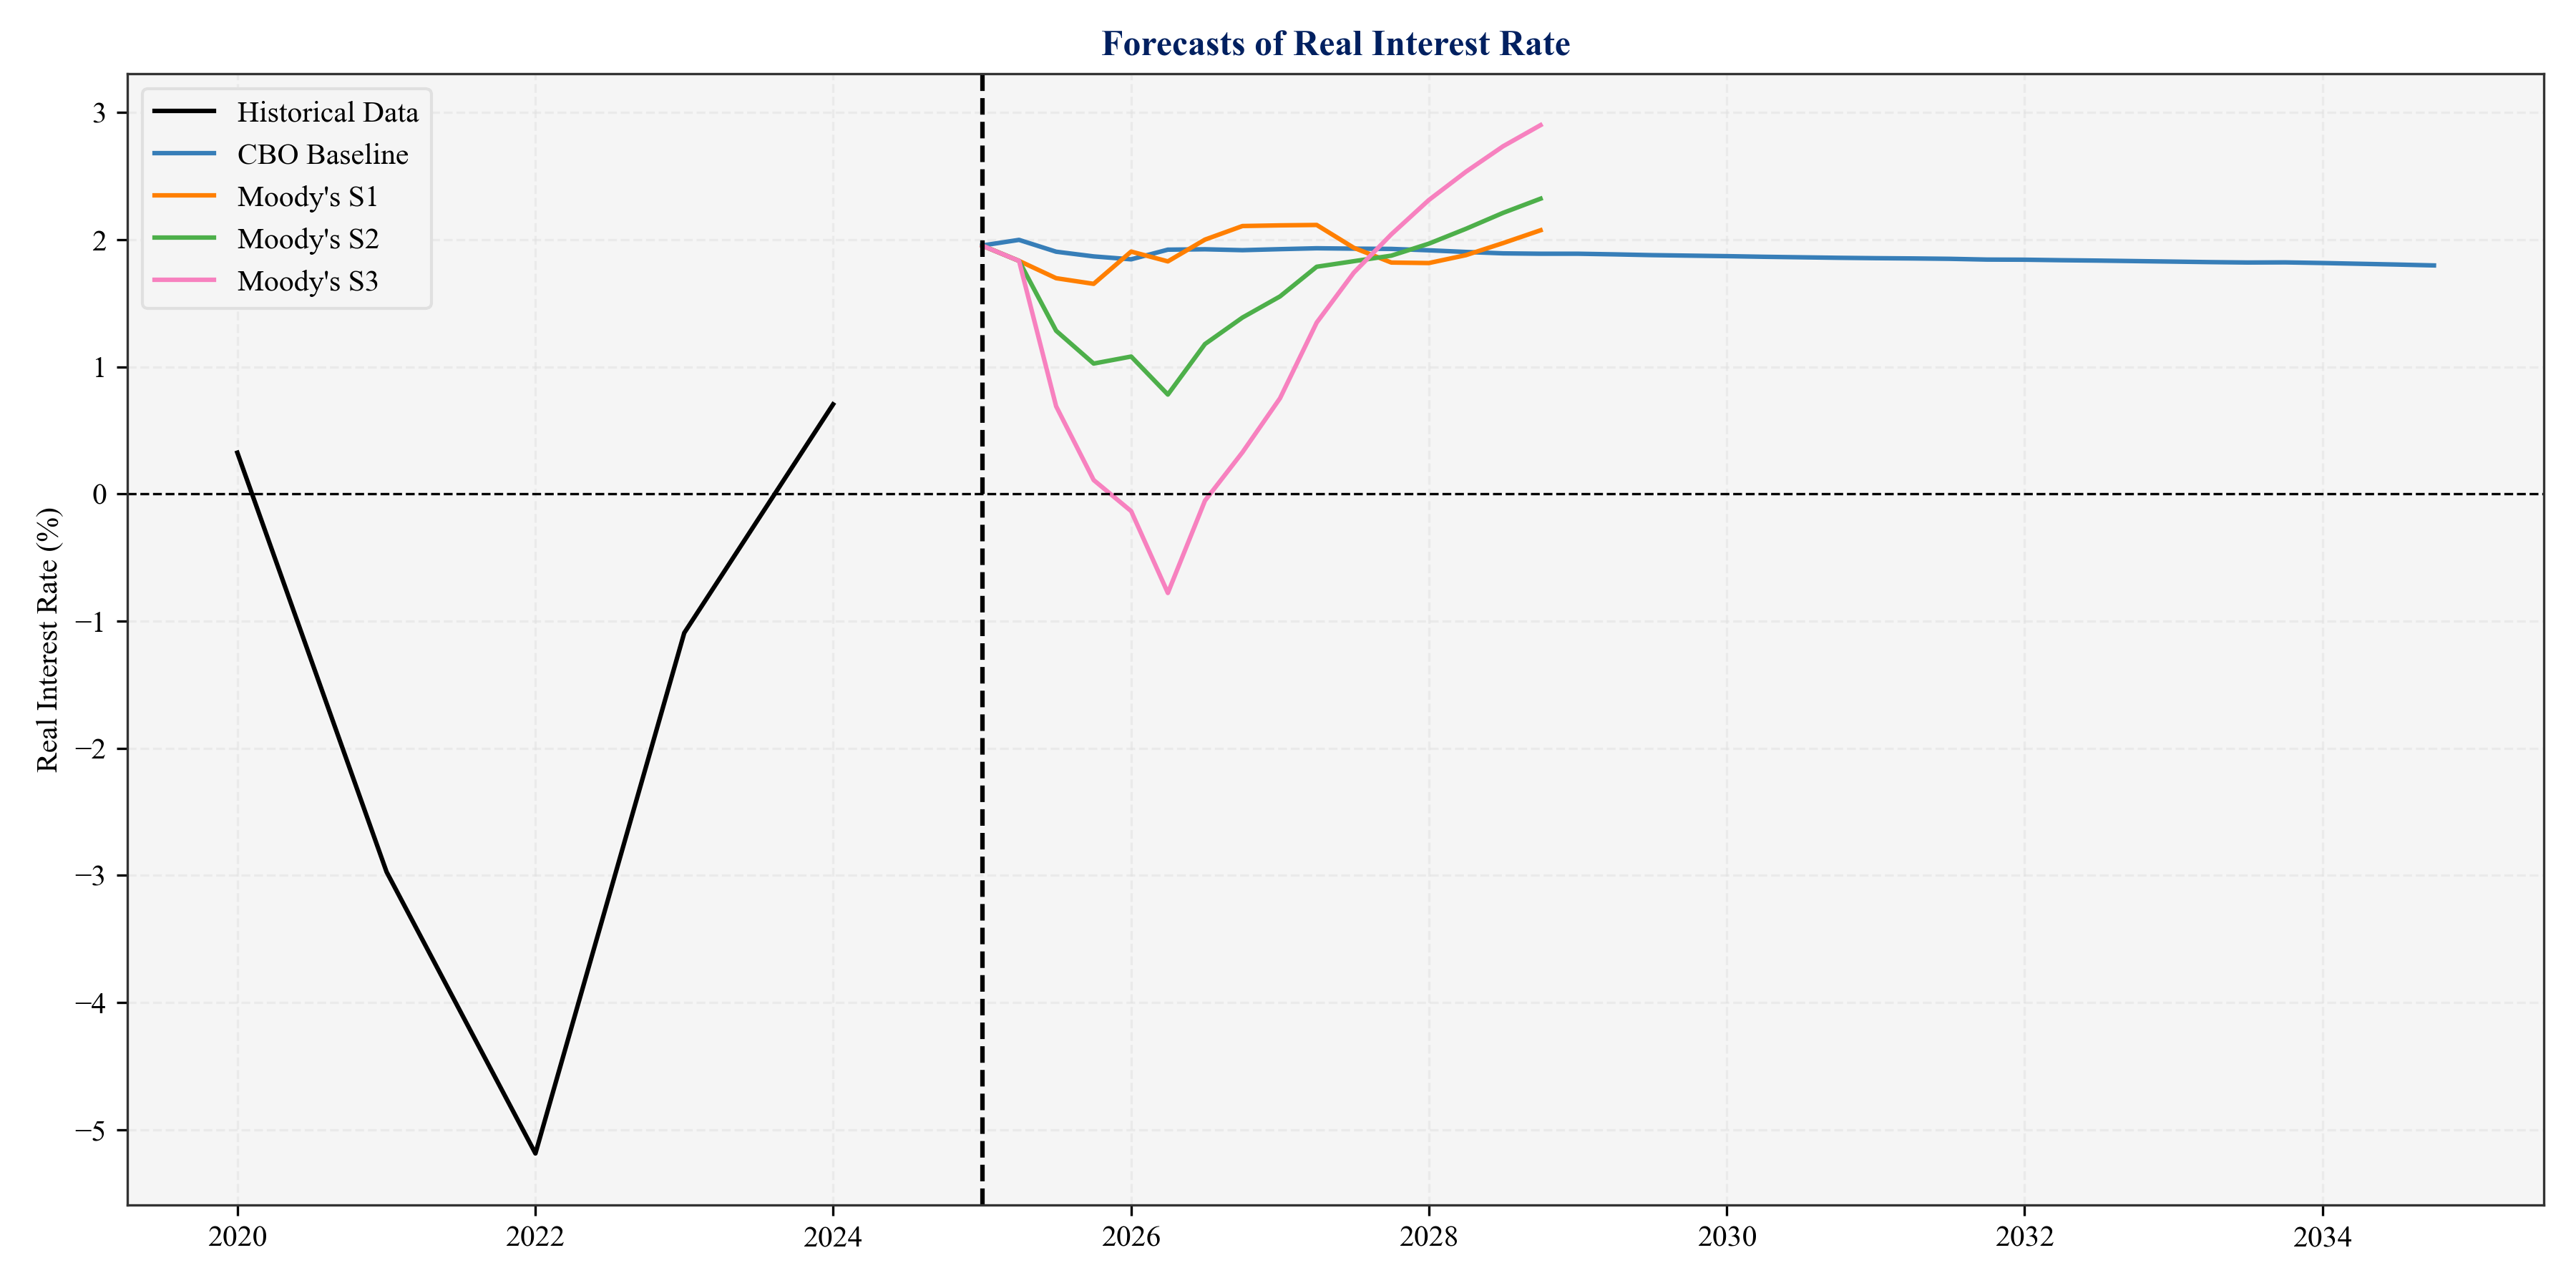
\includegraphics[width=\textwidth]{forecasts_r.png}
    \caption{There is significant heterogeneity across real interest rate projections}
    \label{fig:forecasts_r}
\end{subfigure}

\vspace{1em}  % optional vertical spacing between subfigures

\begin{subfigure}[b]{0.60\textwidth}
    \centering
    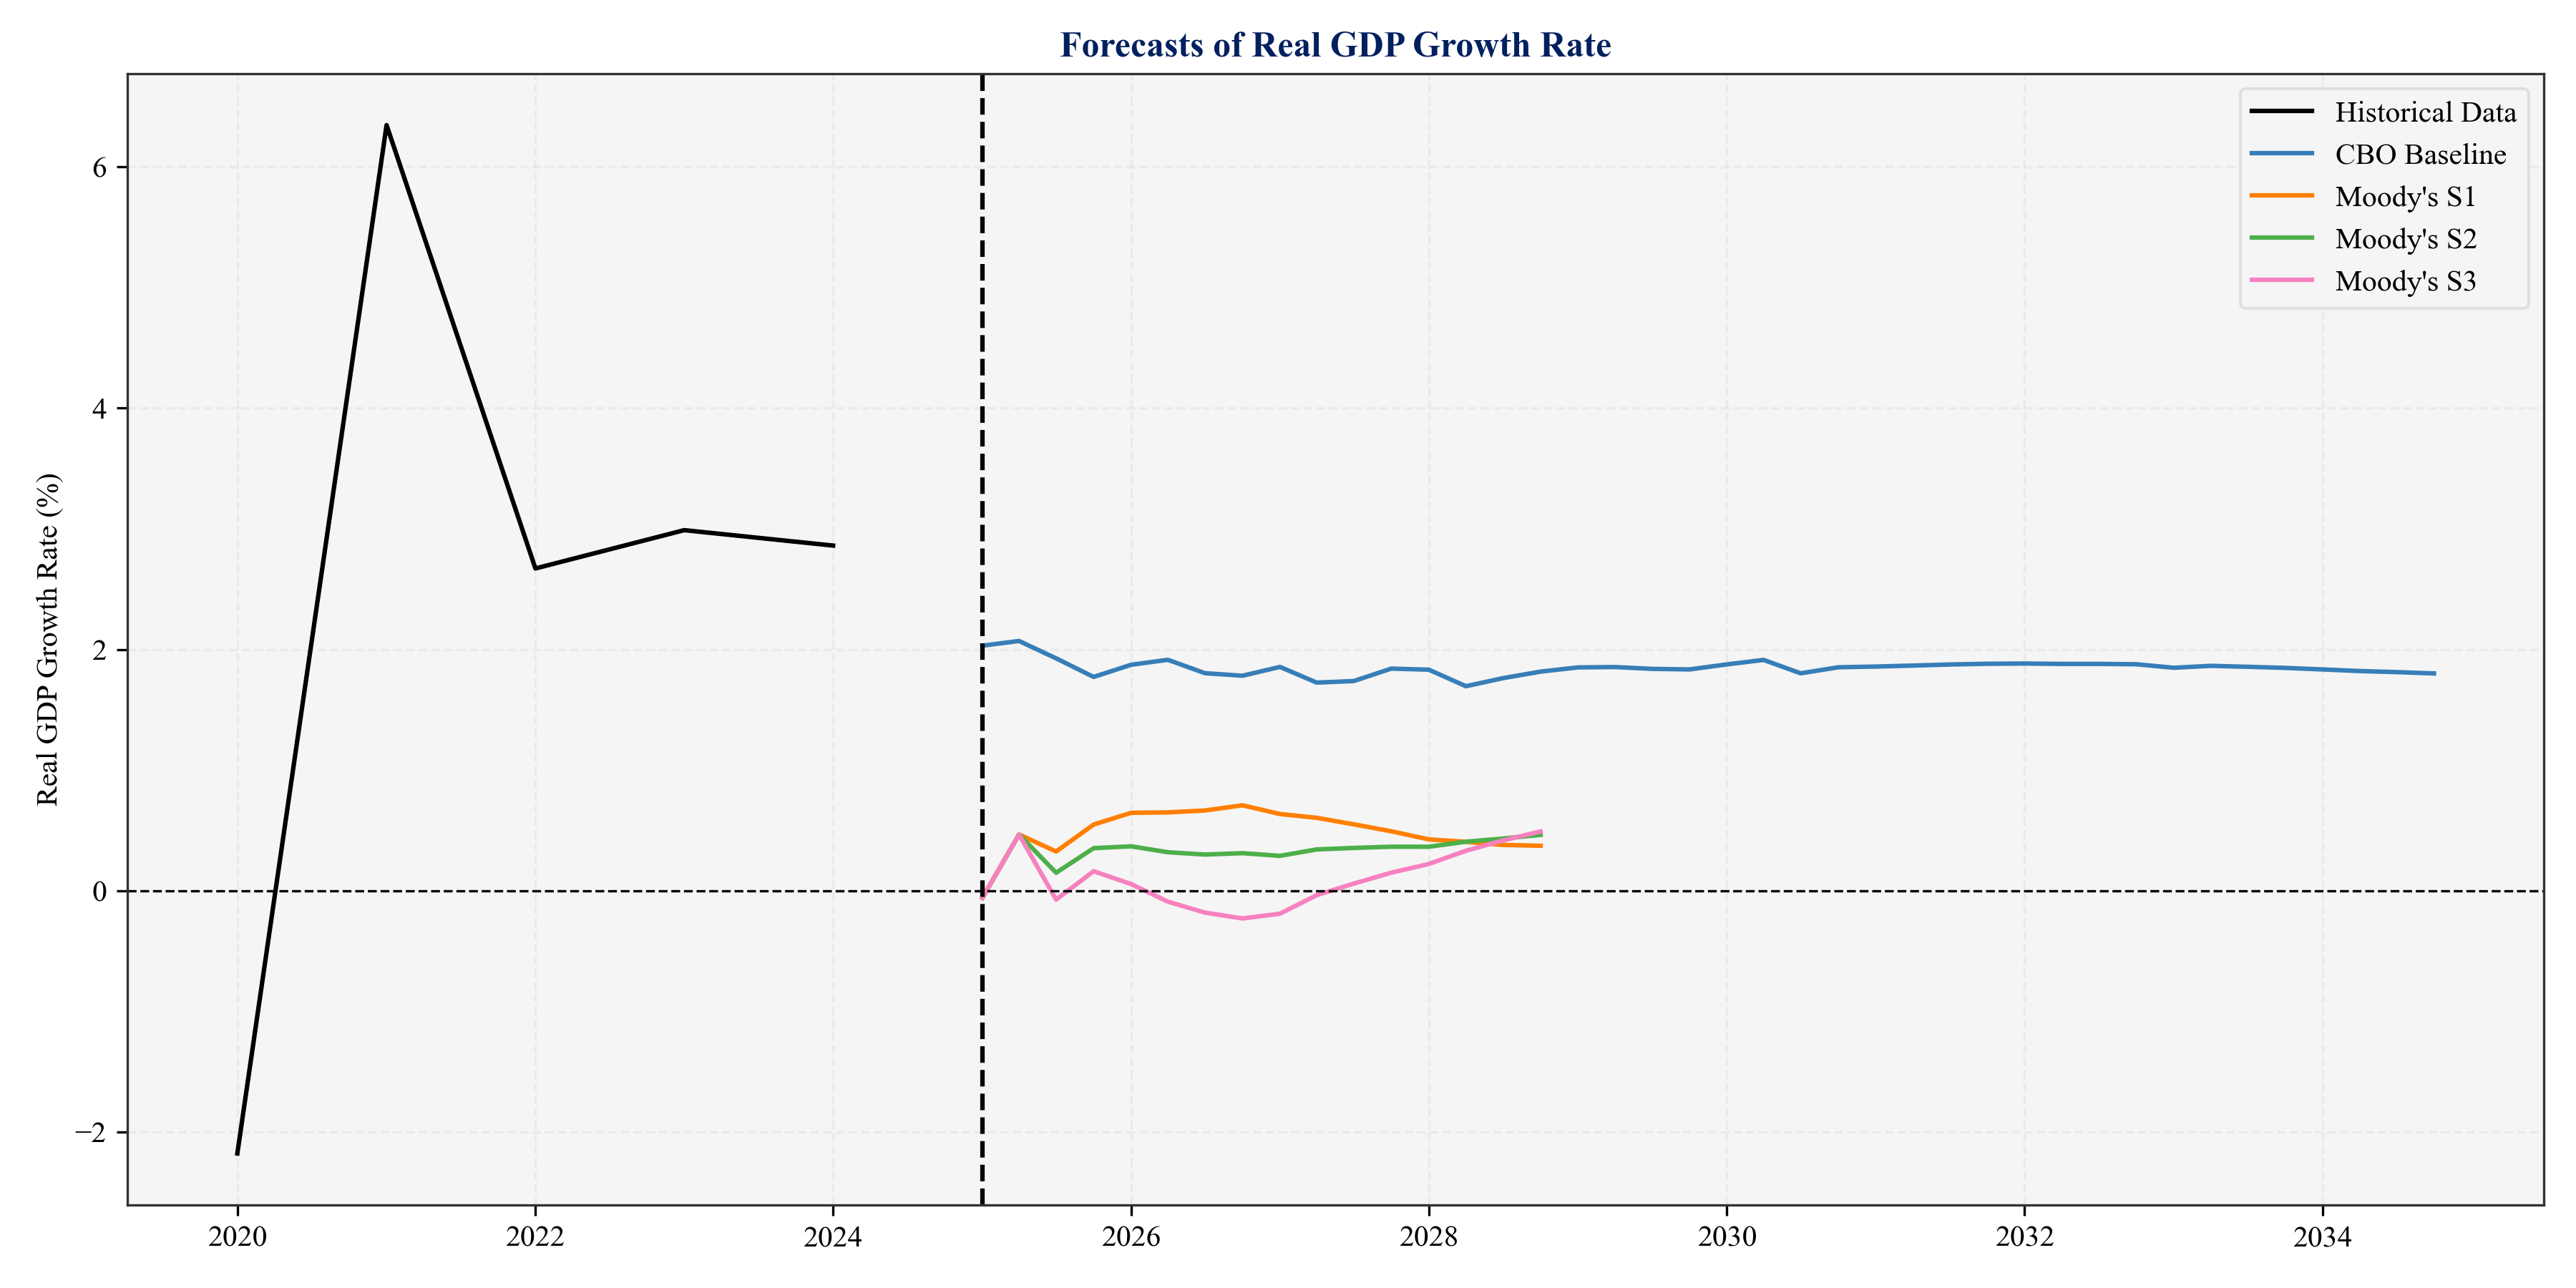
\includegraphics[width=\textwidth]{forecasts_g.png}
    \caption{There is significant heterogeneity across real growth rate projections}
    \label{fig:forecasts_g}
\end{subfigure}

\vspace{1em}

\begin{subfigure}[b]{0.60\textwidth}
    \centering
    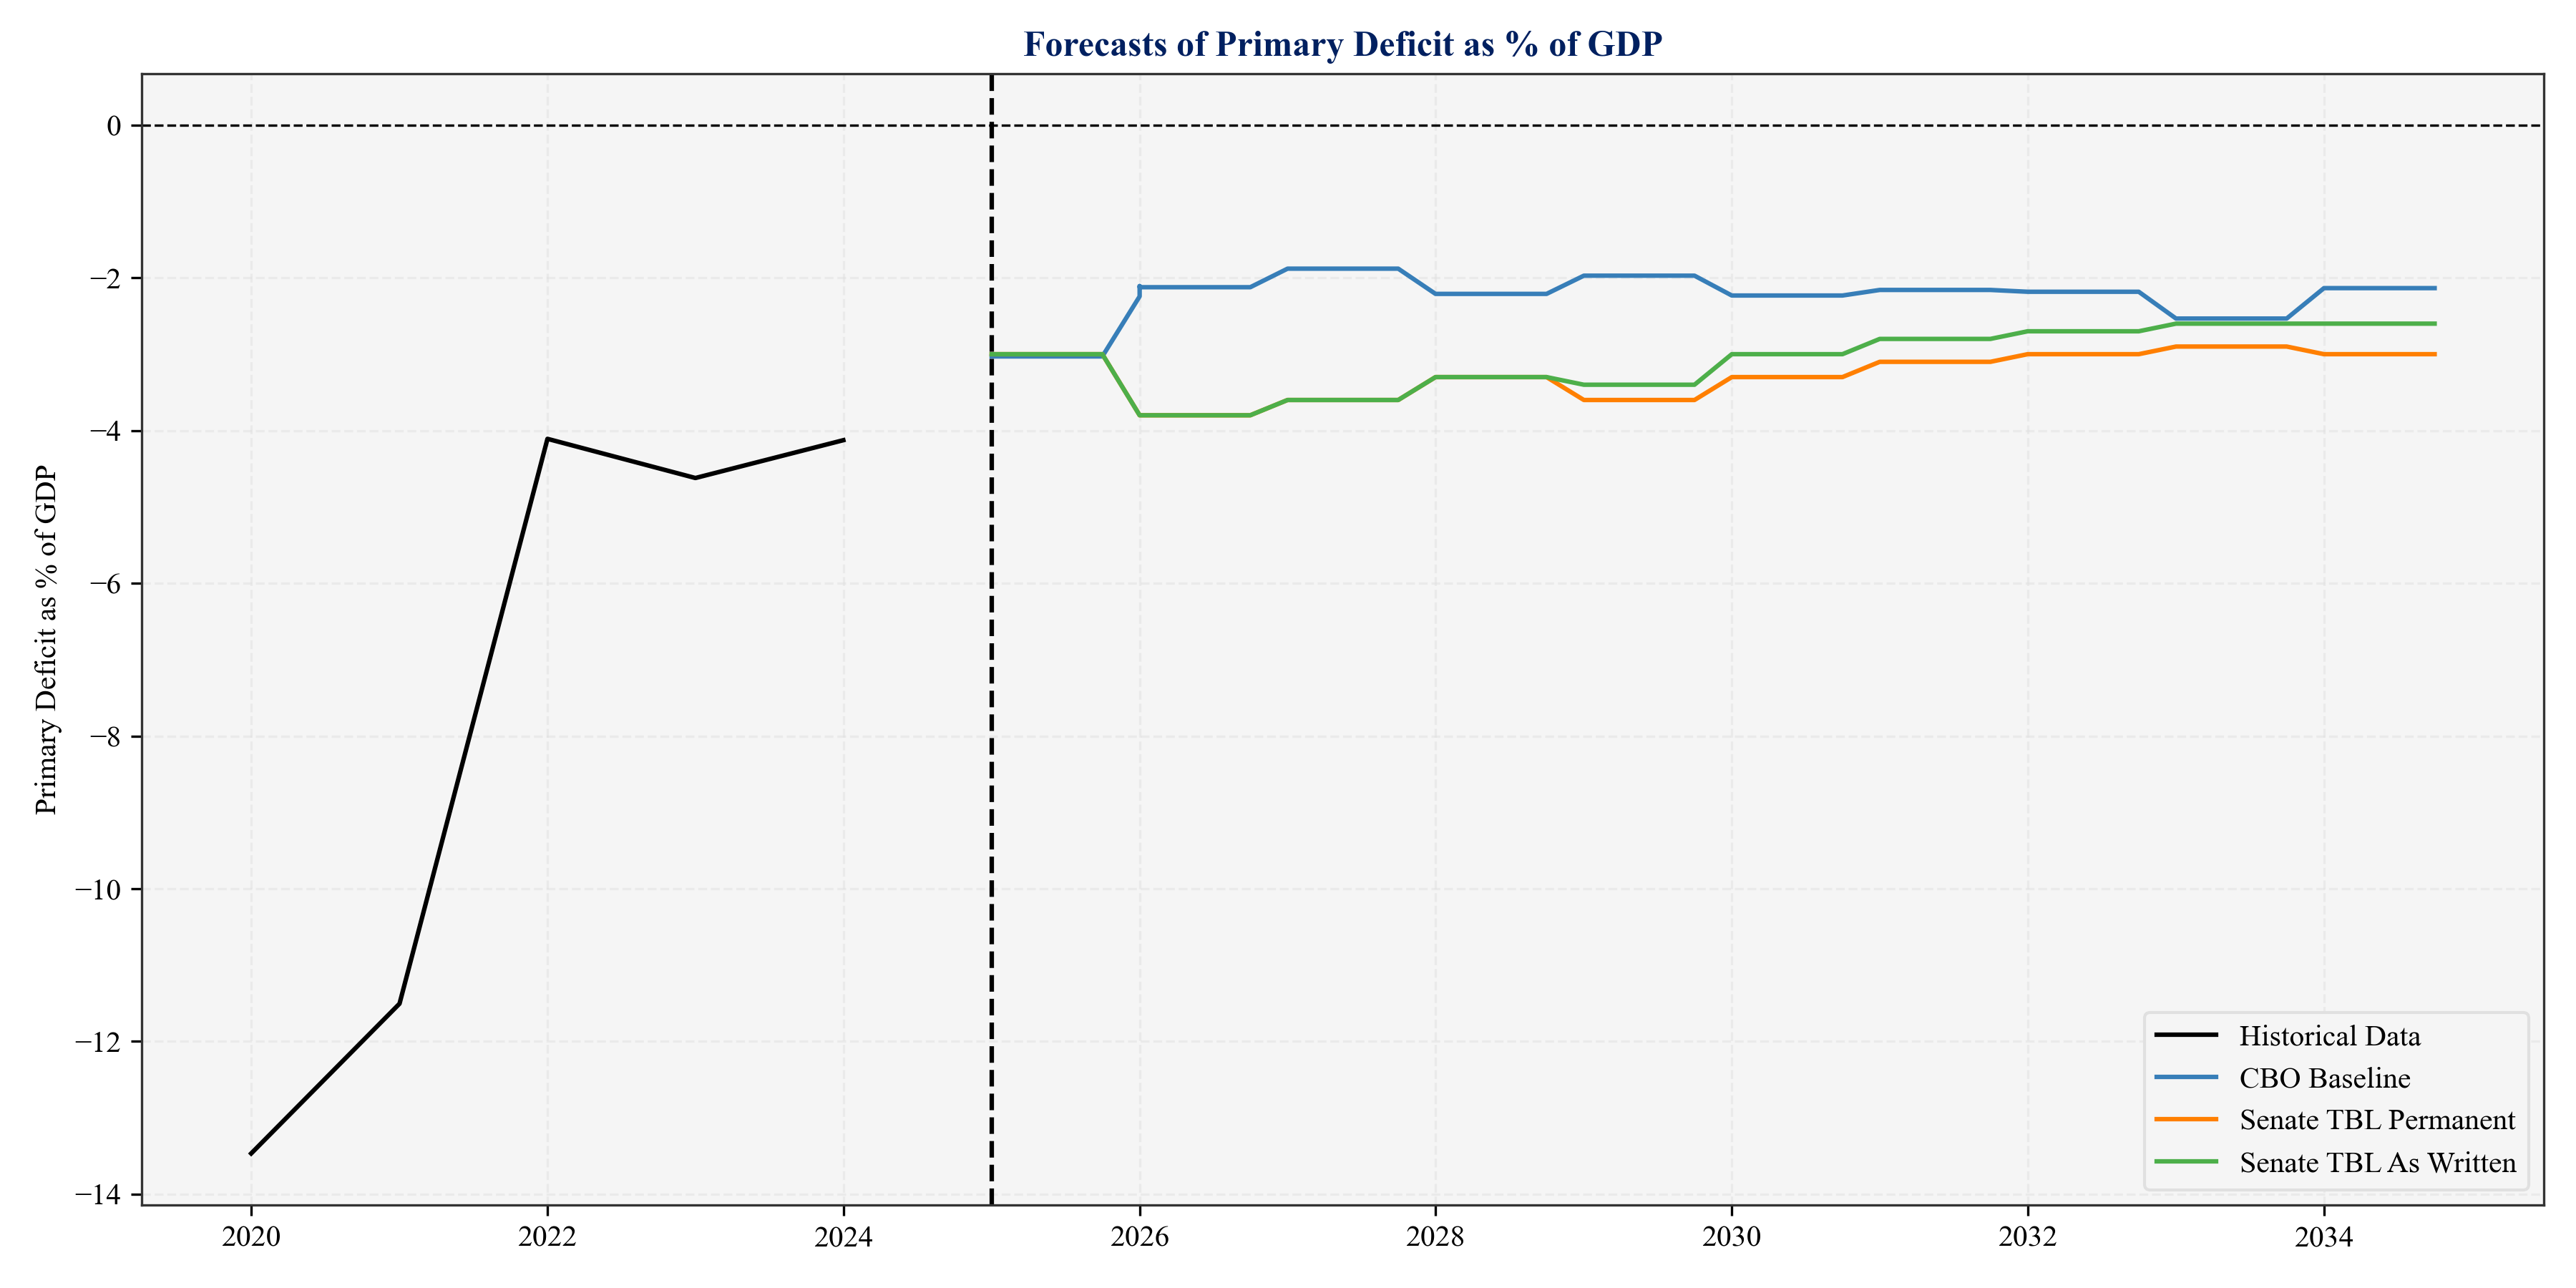
\includegraphics[width=\textwidth]{forecasts_s.png}
    \caption{There is significant heterogeneity across primary deficit projections}
    \label{fig:forecasts_s}
\end{subfigure}

\caption{Forecast heterogeneity across key macroeconomic inputs}
\label{fig:forecasts_all}
\end{figure}

\subsection{Determining Covariation Between Macroeconomic Indicators}

Then, while a choice among these forecasts can give us the first moment, mean, of the distribution of future values for $r$, $g$, and $s$, we have to adopt some assumptions to find the joint distributions. This leaves us with several possibilities. First, we can use historical data to estimate correlations between $r$, $g$, and $s$. Then, the critical assumption to make is what time period. It's clear that the relationship between $r$, $g$, and $s$ varies over time due to structural changes in capital markets, the US economy, and the global economy. By choosing any time period, we would be making an argument about what we think the relationship between these estimates will be in the future. 

To illustrate this, I ran the following simple univariate regressions, using time-varying samples of data. 
\begin{gather}
	r_t = \beta_{r, g} g_t + \epsilon \\
	r_t = \beta_{r, s} s_t + \epsilon \\
	g_t = \beta_{g, r} r_t + \epsilon \\
	g_t = \beta_{g, s} s_t + \epsilon \\
	s_t = \beta_{s, r} r_t + \epsilon \\
	s_t = \beta_{s, g} g_t + \epsilon
\end{gather}

So, in Figure \ref{fig:rolling_betas}, the value for, say $\hat{\beta_{r, g}}$ in year 1985, is equal to the value of $\hat{\beta_{r, g}}$ when estimated using the sample of values for $r$ and $g$ ranging from 1985 to the present. Then, the value of $\hat{\beta_{r, g}}$ in year 1993 is equal to the estimated value of $\hat{\beta_{r, g}}$ when estimated using the sample of values for $r$ and $g$ ranging from 1993 to the present. I also add confidence bends to signify the 95\% confidence interval of $\hat{\beta}$. 

\begin{figure}[htbp!]
\centering
	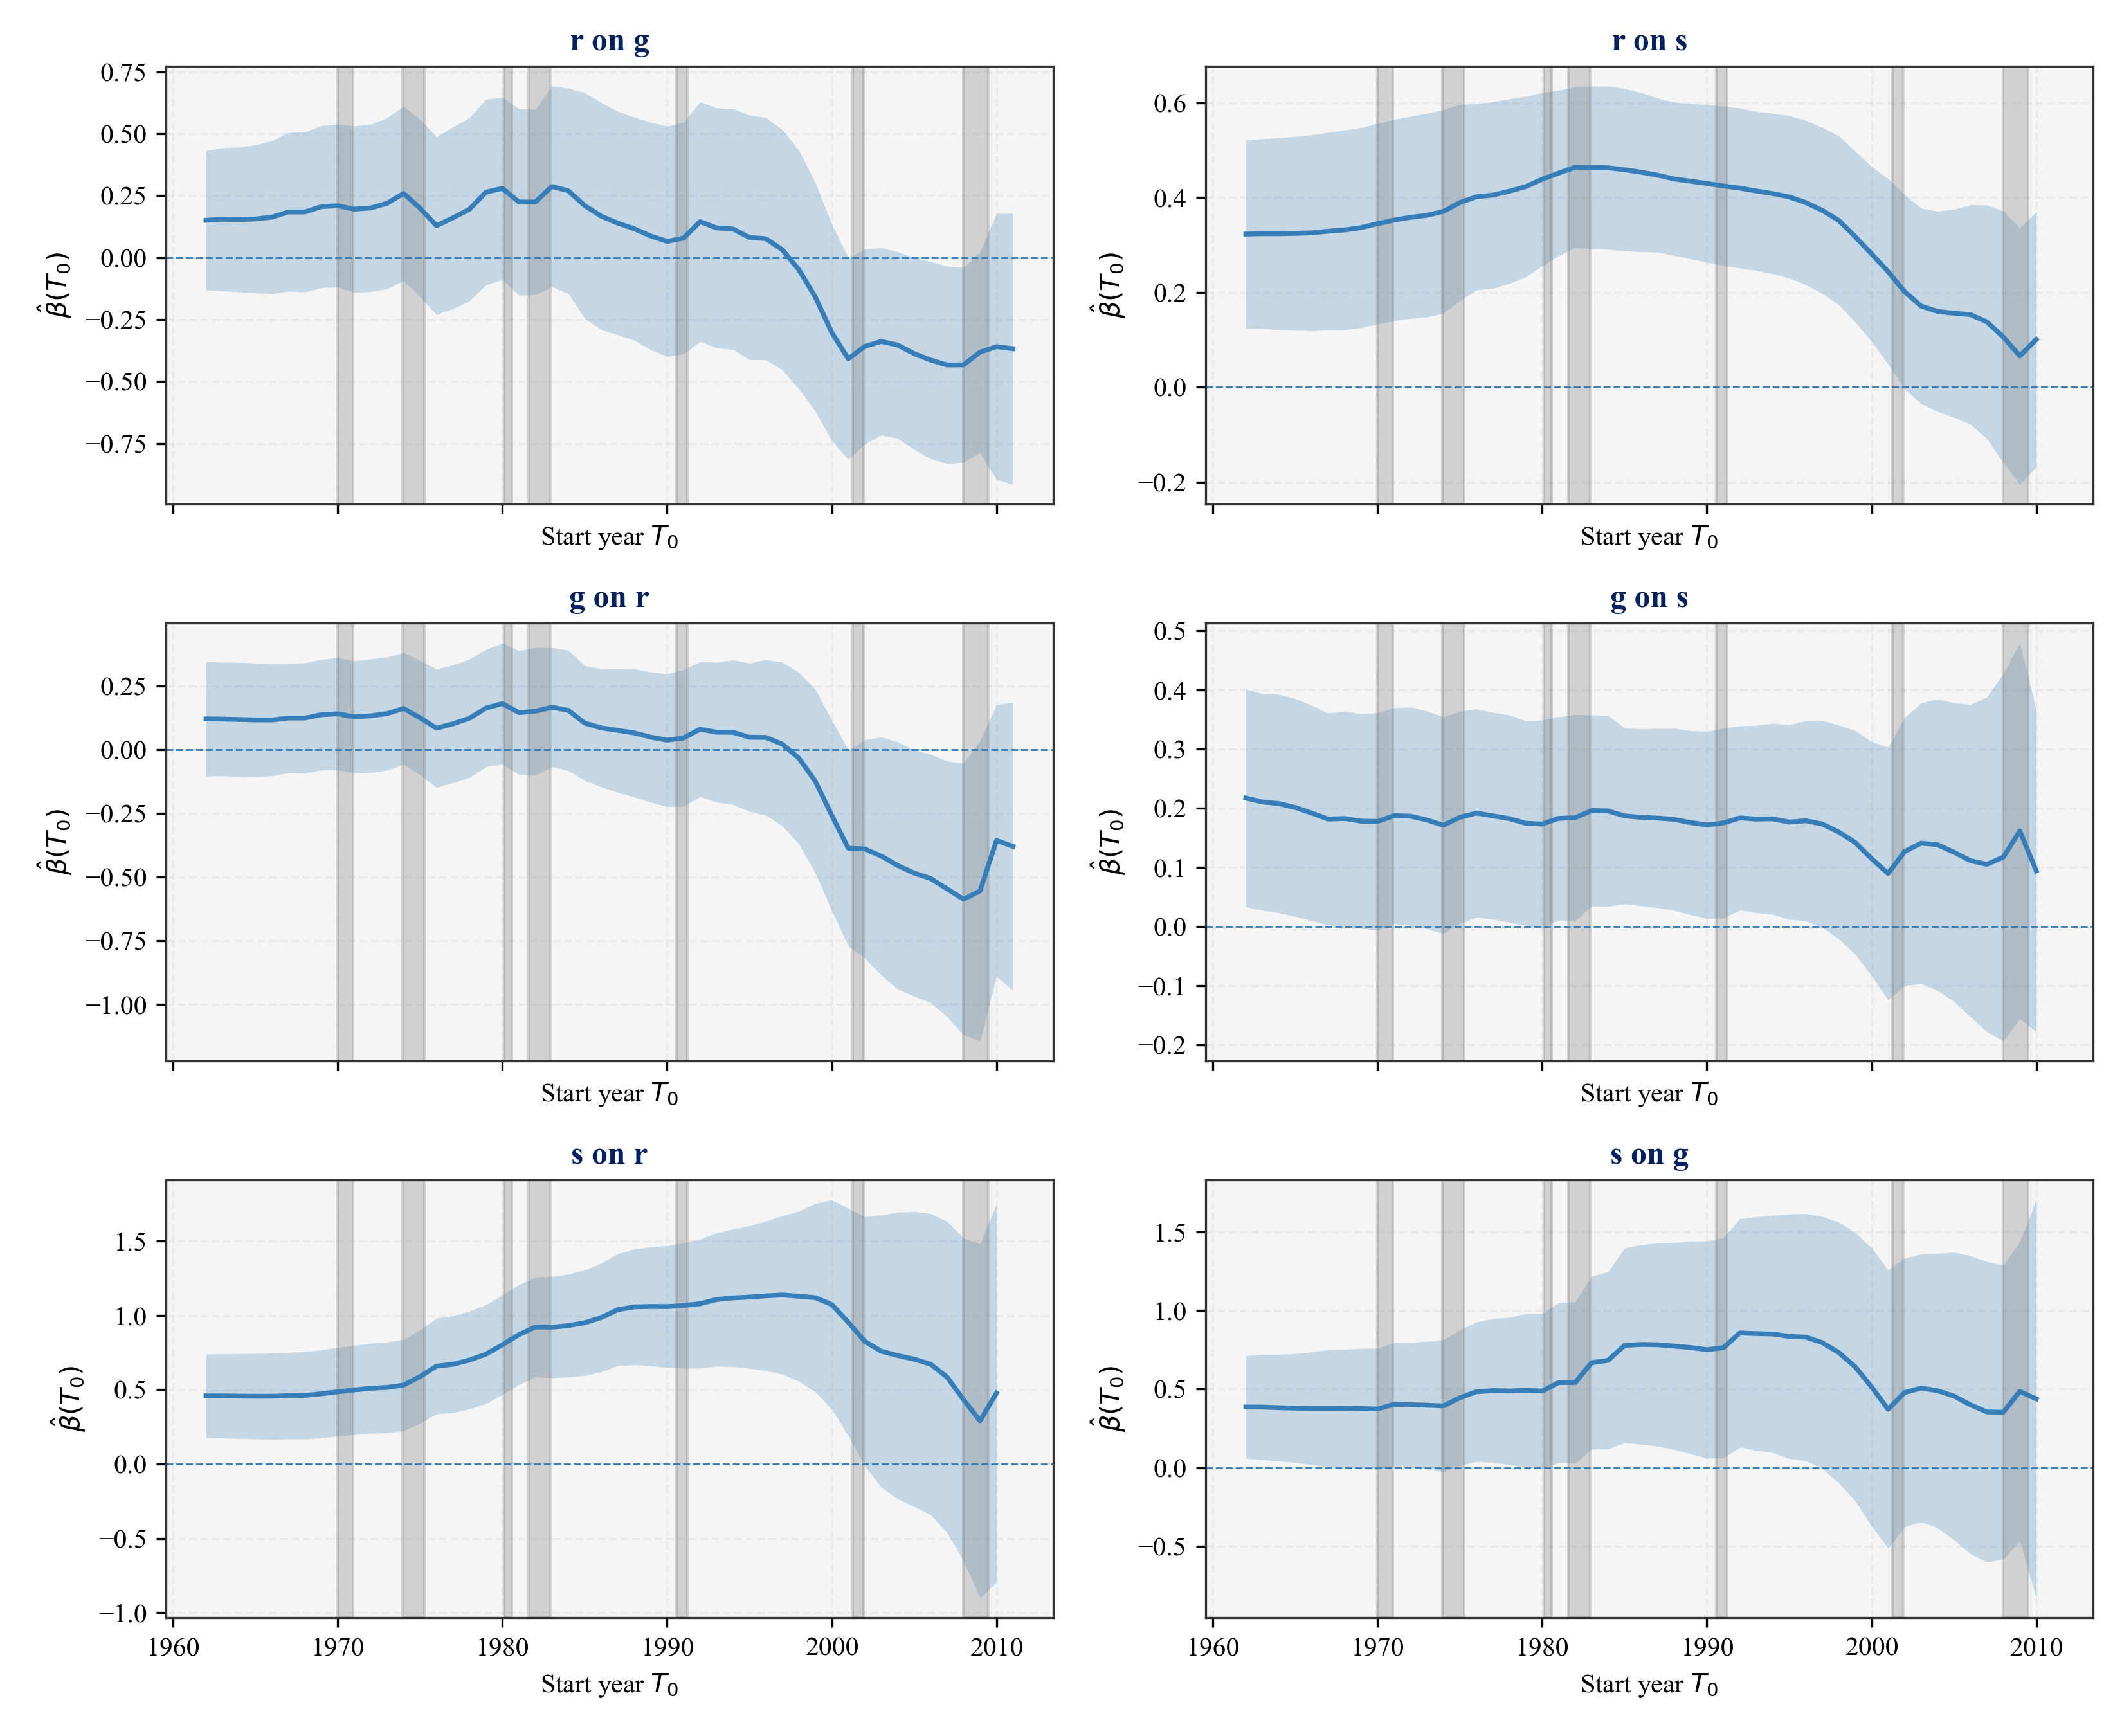
\includegraphics[width=0.8\textwidth]{rolling_betas.png}
\caption{Correlation between our key macroeconomic variables exhibits significant temporal heterogeneity}
\label{fig:rolling_betas}
\end{figure}

From Figure \ref{fig:rolling_betas}, we can make a few observations. First, most of the association between macroeconomic variables are not statistically different from zero, except for 1) $g$ on $s$ and 2) $r$ and $s$ (and vice-versa for each relationship). From this growth has a mostly positive association with the primary surplus, which mechanically makes sense, as GDP is the denominator of $s$. Interestingly, we \textit{do} see a positive relationship between $s$ and $r$; however, if we restrict the universe of data points to only 2000 and onwards, this relationship because statistically indistinguishable from 0. This would re-affirm our argument that post-2000, in particular, we have entered a different fiscal and monetary regime, in which debt/deficit have become decoupled from interest rates. 

\subsection{Selecting $n$}

\end{document}